\documentclass{beamer}
%
% Choose how your presentation looks.
%
% For more themes, color themes and font themes, see:
% http://deic.uab.es/~iblanes/beamer_gallery/index_by_theme.html
%
\mode<presentation>
{
  \usetheme{default}      % or try Darmstadt, Madrid, Warsaw, ...
  \usecolortheme{default} % or try albatross, beaver, crane, ...
  \usefonttheme{default}  % or try serif, structurebold, ...
  \setbeamertemplate{navigation symbols}{}
  \setbeamertemplate{caption}[numbered]
} 
\addtobeamertemplate{navigation symbols}{}{%
	\usebeamerfont{footline}%
	\usebeamercolor[fg]{footline}%
	\hspace{1em}%
	\insertframenumber/\inserttotalframenumber
}
\setbeamertemplate{footline}{
	\hbox{%
		\begin{beamercolorbox}[wd=\paperwidth,ht=3ex,dp=1.5ex,leftskip=2ex,rightskip=2ex]{page footer}%
			\usebeamerfont{title in head/foot}%
			\insertshorttitle \hfill
			\insertsection \hfill
			\insertframenumber{} / \inserttotalframenumber
	\end{beamercolorbox}}%
}
\usepackage[english]{babel}
\usepackage[utf8x]{inputenc}
\usepackage{xcolor} % For textcolor
\usepackage{pgfplots} % For Tikz
\usepackage{media9}
\usepackage{tikz}
\usetikzlibrary{shapes,arrows}

\title[]{Control Architectures for Distributed Control of Mobile Robots}
\author{\textbf{Adwait Datar}}
\institute{Institute of Control Systems\\ Technical University of Hamburg\\ \vspace{1cm}CPN Workshop, Dec-2020\\ \vspace{1cm}This work was funded by the German Research Foundation (DFG) within their priority programme SPP 1914 Cyber-Physical Networking.}
\date{}
 \AtBeginSection[]
 {
 	\begin{frame}
 	\frametitle{Table of Contents}
 	\tableofcontents[currentsection]
	 \end{frame}
 } 

\begin{document}
\begin{frame}	
  \titlepage
\end{frame}

%Uncomment these lines for an automatically generated outline.
%\begin{frame}{Outline}
% \tableofcontents
%\end{frame}
%%%%%%%%%%%%%%%%%%%%%%%%%%%%%%%%%%%%%%%%%%%%%%%%%%%%%%%%%%%%%%%%%%%%%
%\begin{frame}{Outline}
%	\begin{itemize}
%		\item[1] Flocking algorithms to address the source-seeking problem
%		\begin{itemize}
%			\item Theory for double integrator agent dynamics
%			\item Experimental results with quadrotors
%			\item \textcolor{blue}{(Speculative)} Extension to non-linear/uncertain agents with
%			\begin{itemize}
%				\item Dissipativity based arguments
%				\item Singular perturbation arguments
%				\item Integral Quadratic Constraints (IQCs)
%			\end{itemize}
%			
%		\end{itemize}
%		\item[2] Formation Stabilization with a decoupled architecture
%		\begin{itemize}
%			\item Decouple	d control architecture
%			\item Theory
%			\item Simulation results
%			\item \textcolor{blue}{(Speculative)} Extension to lossy networks with
%			\begin{itemize}
%				\item Information flow filter as a Markov Jump Linear System (MJLS)
%			\end{itemize}
%		\end{itemize}
%	\end{itemize}
%\end{frame}
%%%%%%%%%%%%%%%%%%%%%%%%%%%%%%%%%%%%%%%%%%%%%%%%%%%%%%%%%%%%%%%%%%%%%
%%%%%%%%%%%%%%%%%%%%%%%%%%%%%%%%%%%%%%%%%%%%%%%%%%%%%%%%%%%%%%%%%%%%%
\begin{frame}{Motivating Scenarios}
    Fukushima Disaster (2011)
    %\footnote{https://rememberfukushima.org/fallout-maps/}
    \hspace{0.4 cm}
    Deep Water Horizon (2010)
    %\footnote{https://response.restoration.noaa.gov}
    \\
	\begin{minipage}{0.45\textwidth}	
		\begin{figure}
			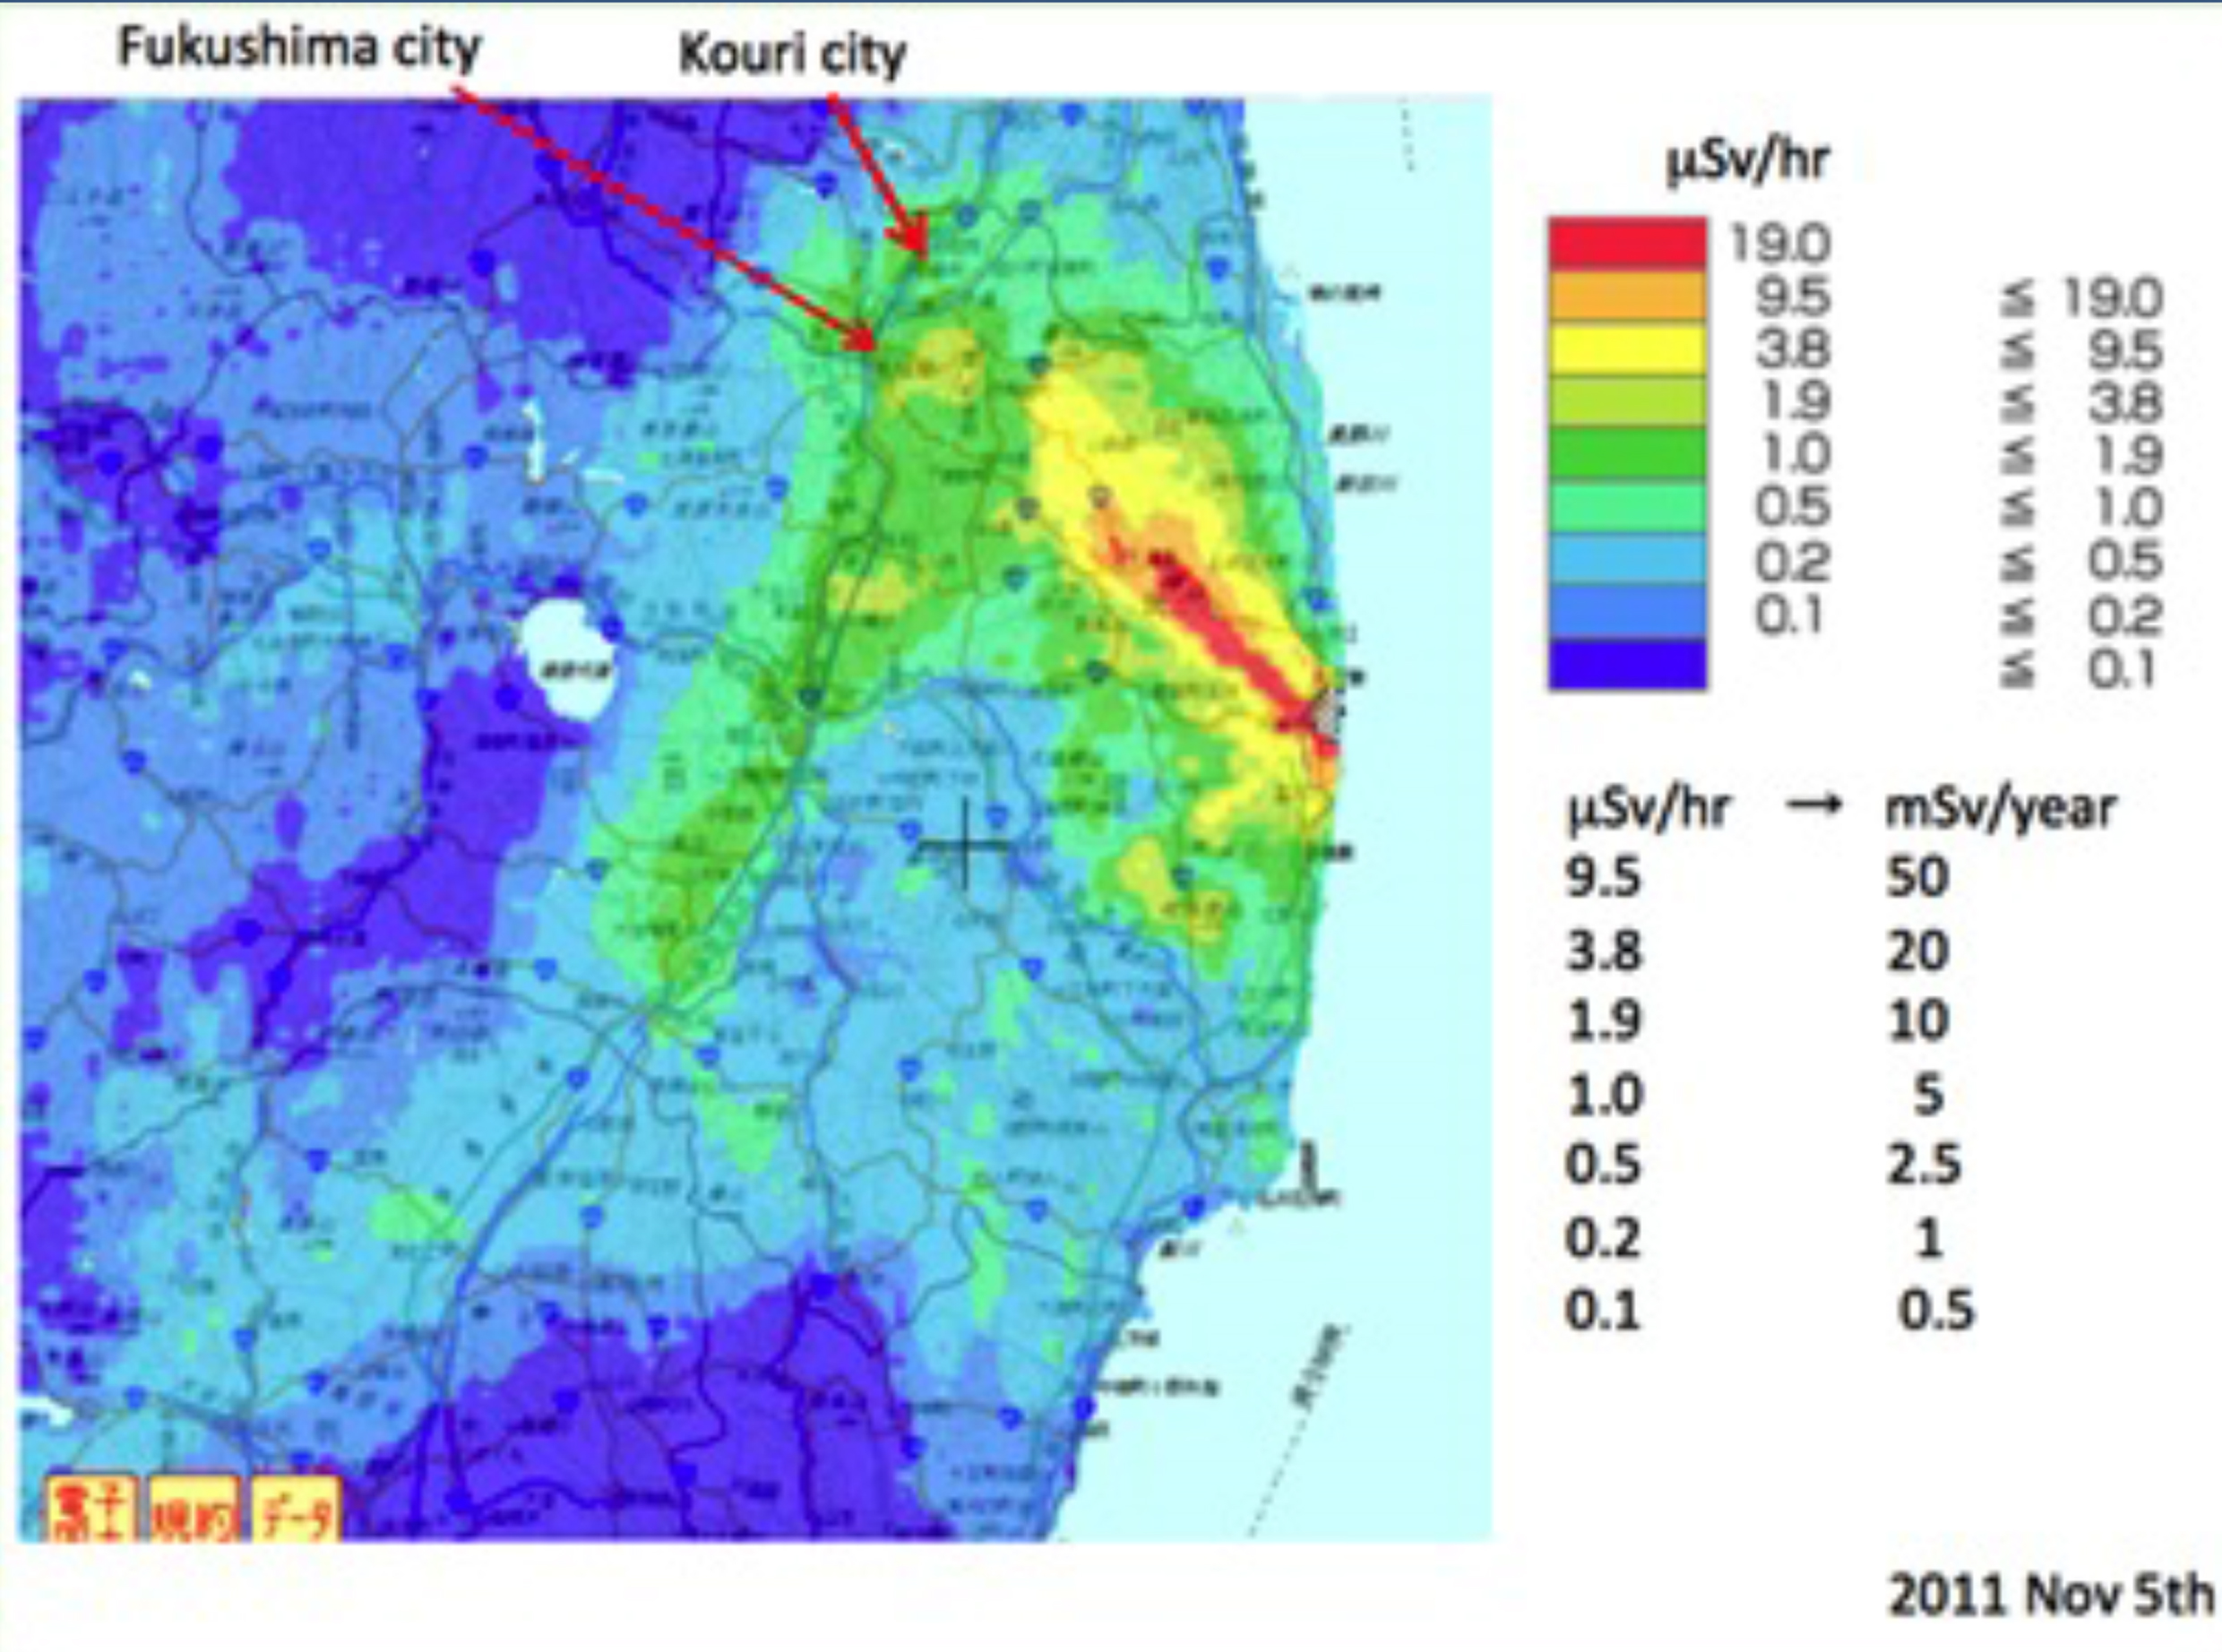
\includegraphics[width=1\textwidth]{figures/fukushima_disaster.jpg}
			%\caption{Fukushima Disaster (2011)}
			%\label{fig:fukushima_disaster}
		\end{figure}
		\begin{figure}
			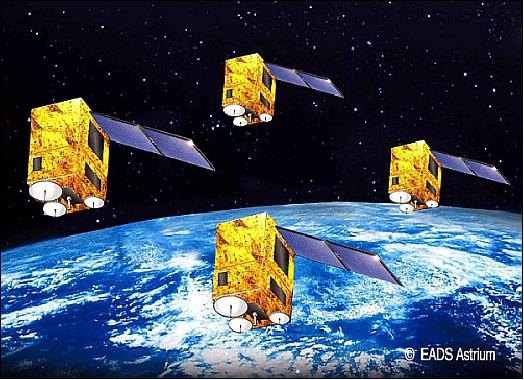
\includegraphics[scale=0.2]{figures/Essaim_constellation.jpg}\label{fig:satellite_flock}
		\end{figure}
	\end{minipage}
	\hspace{0.05cm}
	\begin{minipage}{0.45\textwidth}
		\begin{figure}
			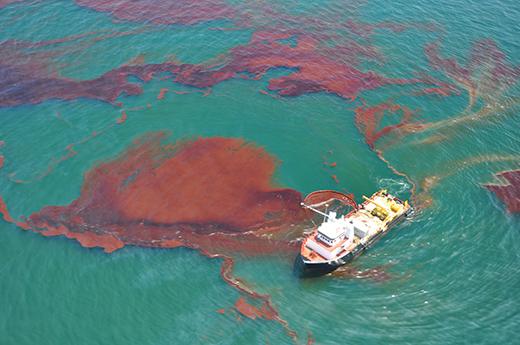
\includegraphics[width=\textwidth]{figures/oil_spill.jpg}
			%\caption{Oil Spills}
			%\label{fig:oilspills}
		\end{figure}
		\begin{figure}
			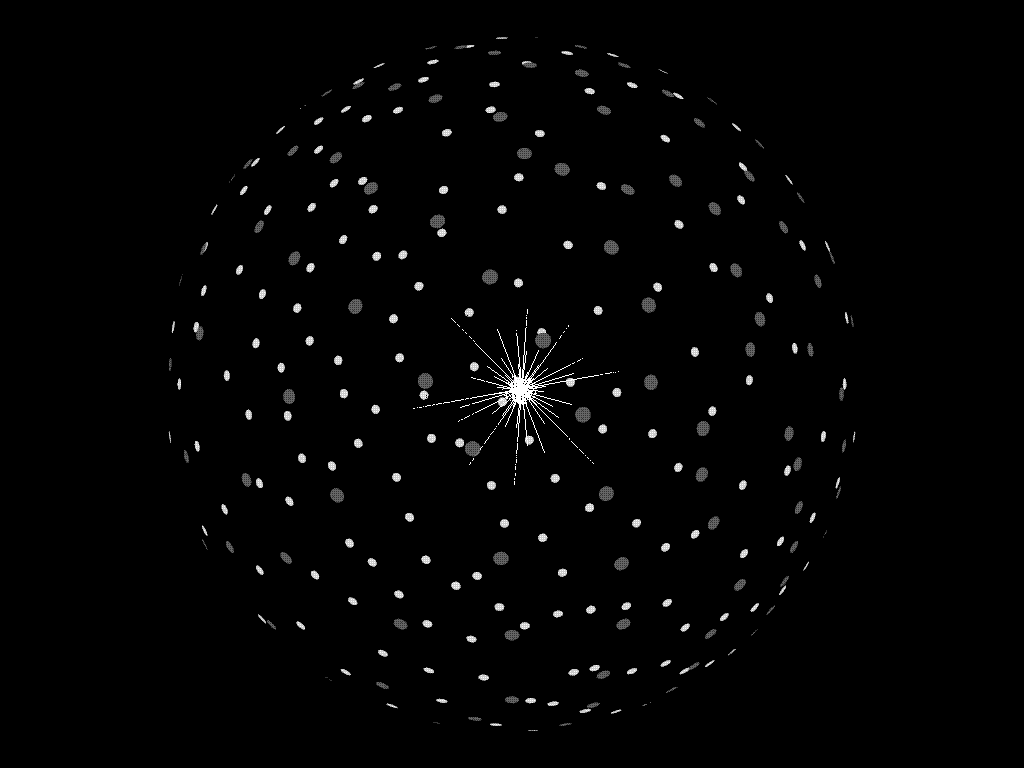
\includegraphics[scale=0.1]{figures/Dyson_swarm.png}		
			\label{fig:Dyson_swarms}
		\end{figure}	
	\end{minipage} 
 .
 \hspace{0.5 cm}
  EADS Astrium 
 %\footnote{https://earth.esa.int}
\hspace{1.7 cm}
Dyson Swarm (Why not !)
\\
\vspace{0.5cm}
\begin{itemize}
	\item Have figures for: Formation forming, flocking, source-seeking, Platooning 
\end{itemize}
\end{frame}
%%%%%%%%%%%%%%%%%%%%%%%%%%%%%%%%%%%%%%%%%%%%%%%%%%%%%%%%%%%%%%%%%%%%%
%%%%%%%%%%%%%%%%%%%%%%%%%%%%%%%%%%%%%%%%%%%%%%%%%%%%%%%%%%%%%%%%%%%%%
\begin{frame}{Physical Agent Dynamics}	
	\begin{itemize}
		\item Crazyflie picture 
		\item Hippo campus picture
		\item Zooids picture
		\item LTI/LPV agents, non-holonomic constraints
	\end{itemize}
\end{frame}
%%%%%%%%%%%%%%%%%%%%%%%%%%%%%%%%%%%%%%%%%%%%%%%%%%%%%%%%%%%%%%%%%%%%%
%%%%%%%%%%%%%%%%%%%%%%%%%%%%%%%%%%%%%%%%%%%%%%%%%%%%%%%%%%%%%%%%%%%%%
\begin{frame}{Core Idea}	
	\begin{itemize}
		\item Control of a single non-linear (possibly non-holonomic) agent: Well-studied problem and various techniques available
		\begin{itemize}
			\item LPV
			\item Dynamic-inversion
			\item Flatness-based control
		\end{itemize}		
		\item About three decades of work on studying interconnections of "simple" agent dynamics where simple could for example be
		\begin{itemize}
			\item single/ double integrators
			\item positive systems 
		\end{itemize} 
	\item Can we maintain this separation in the controller design? i.e design local agent controllers and study the interconnections of these closed loop systems
	\item Can we give some stability and performance guarantees with such a strategy?
	\item What kind of control architectures are possible?
	\end{itemize}
\end{frame}
%%%%%%%%%%%%%%%%%%%%%%%%%%%%%%%%%%%%%%%%%%%%%%%%%%%%%%%%%%%%%%%%%%%%%
%%%%%%%%%%%%%%%%%%%%%%%%%%%%%%%%%%%%%%%%%%%%%%%%%%%%%%%%%%%%%%%%%%%%%
\begin{frame}{Different Control Architectures}	
	\begin{minipage}{0.45\textwidth}	
		\begin{figure}
			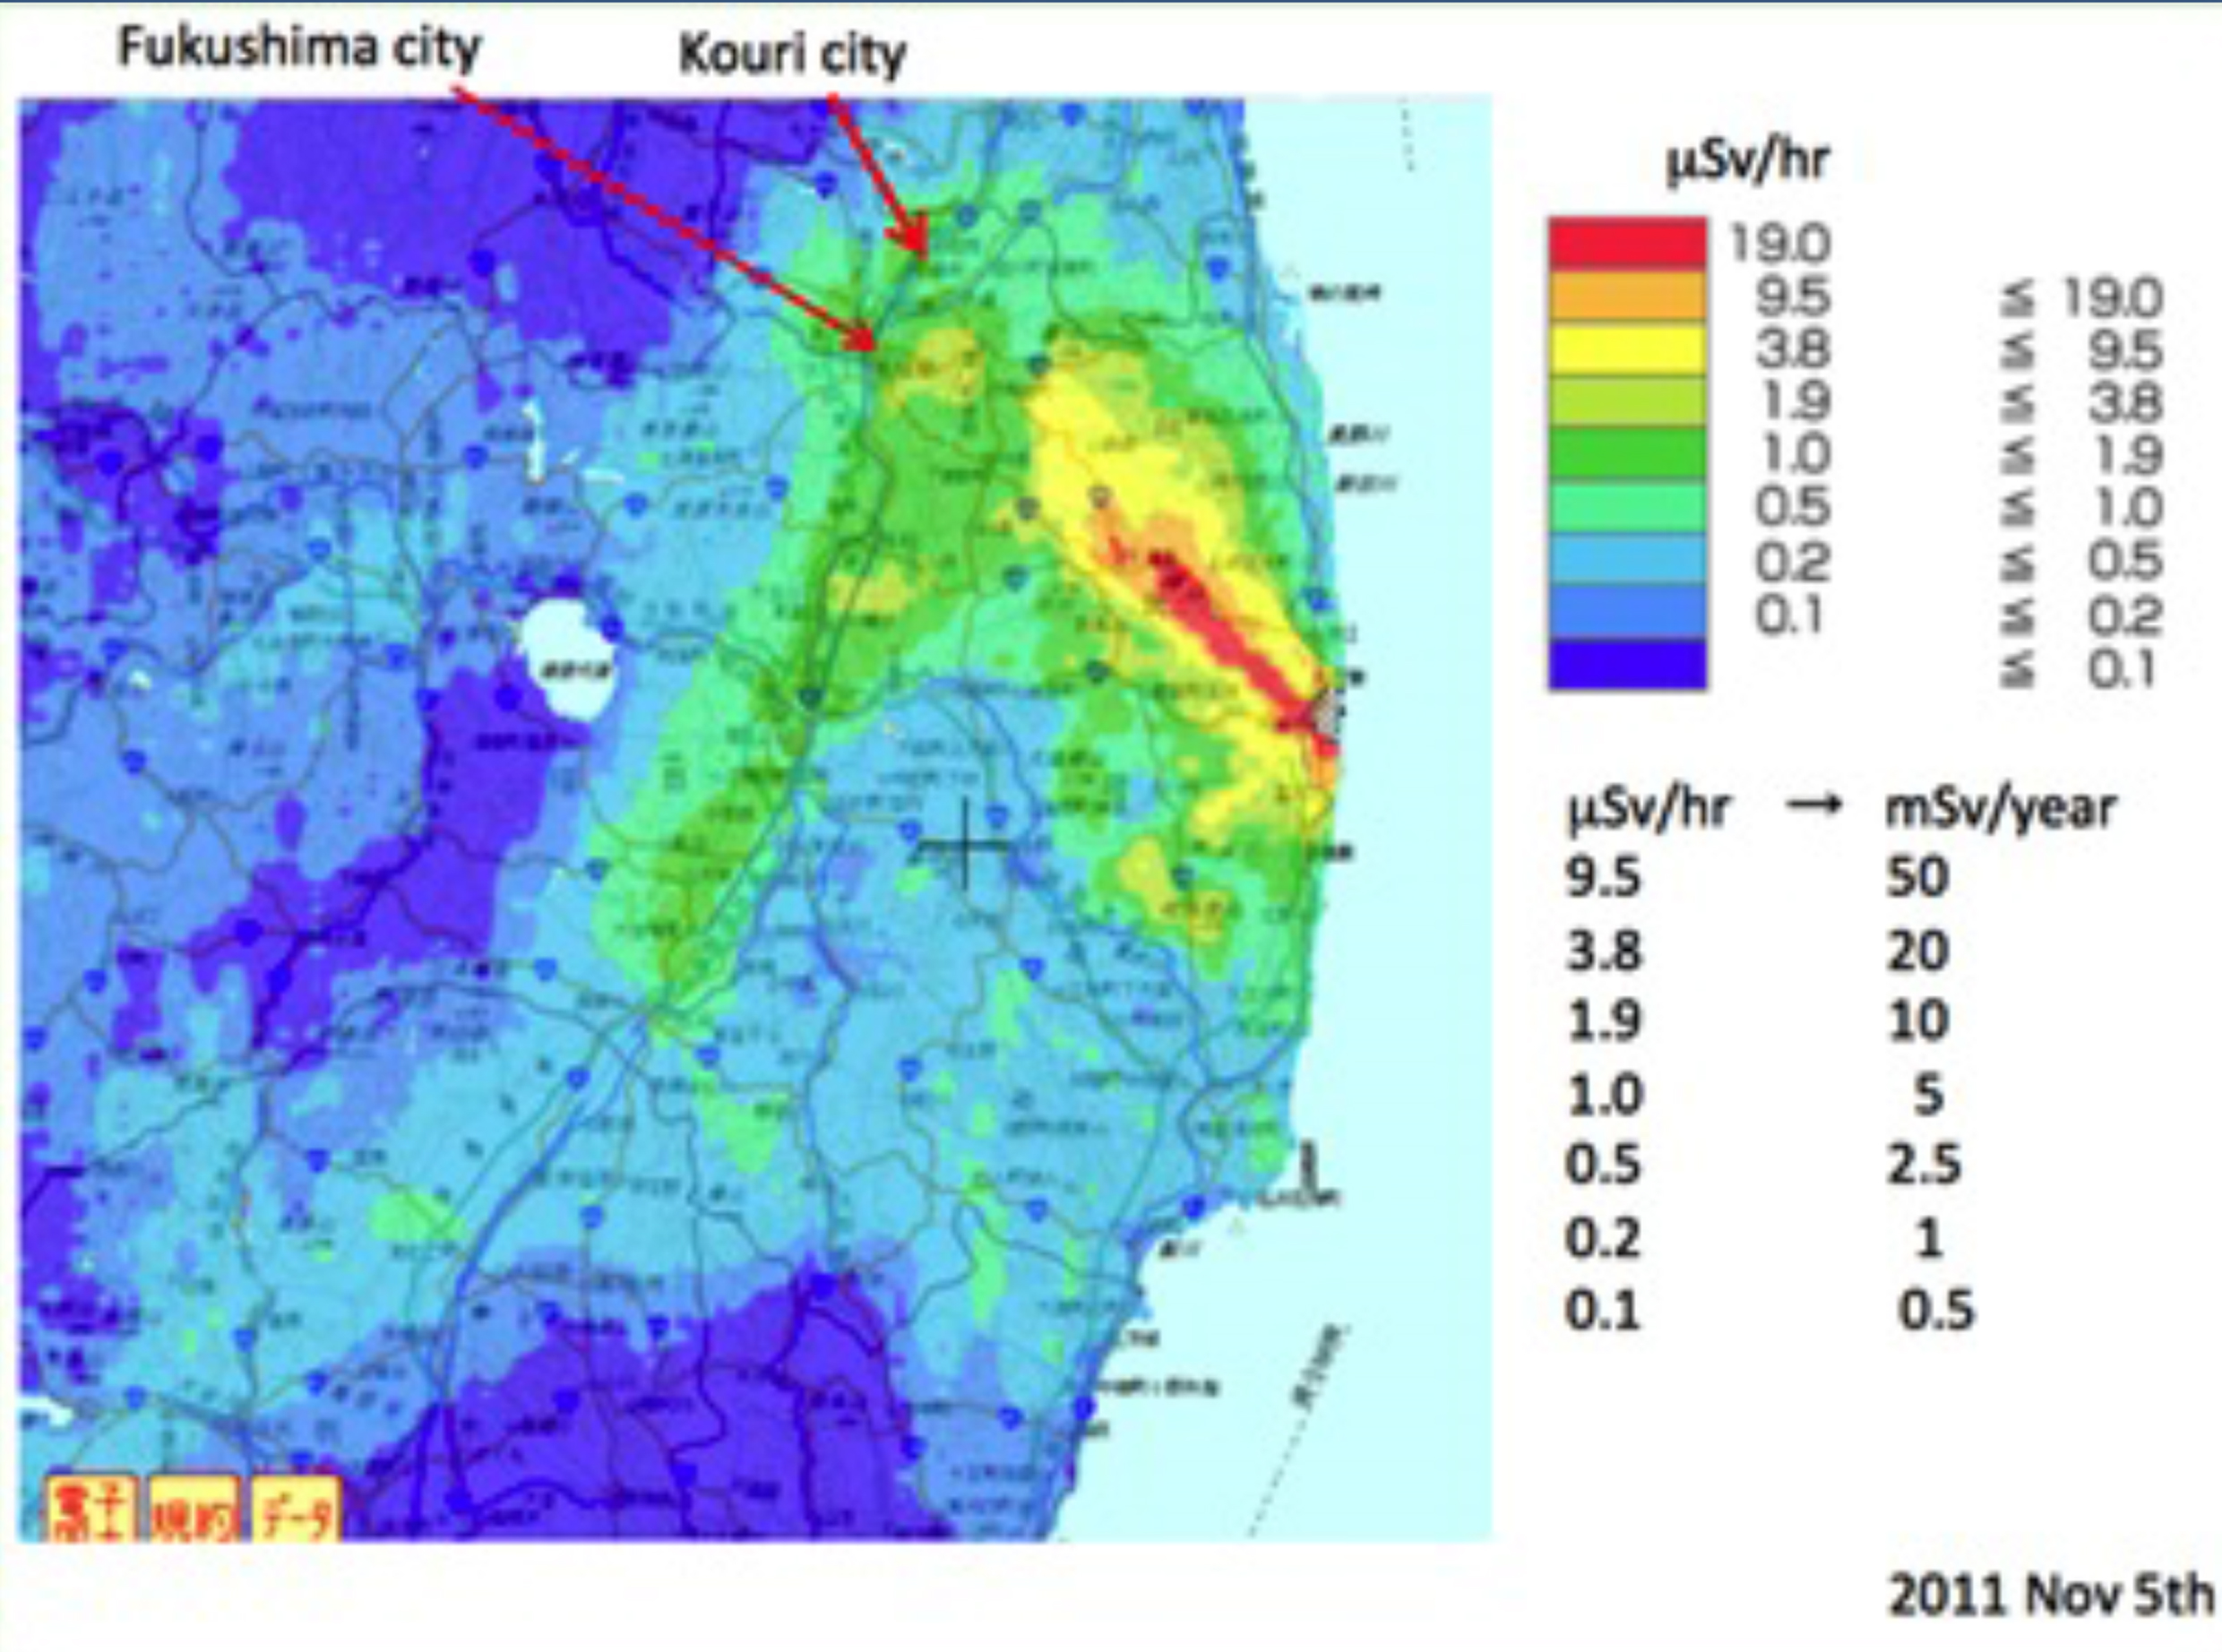
\includegraphics[width=1\textwidth]{figures/fukushima_disaster.jpg}
			%\caption{Fukushima Disaster (2011)}
			%\label{fig:fukushima_disaster}
		\end{figure}
		Coupled architecture
		\begin{itemize}
		\item Maintenance of relative positions important (e.g asdf) 
		\item inter-agent distances are low
		\item High disturbances
		\end{itemize}
	\end{minipage}
	\hspace{0.05cm}
	\begin{minipage}{0.45\textwidth}
			\begin{figure}
			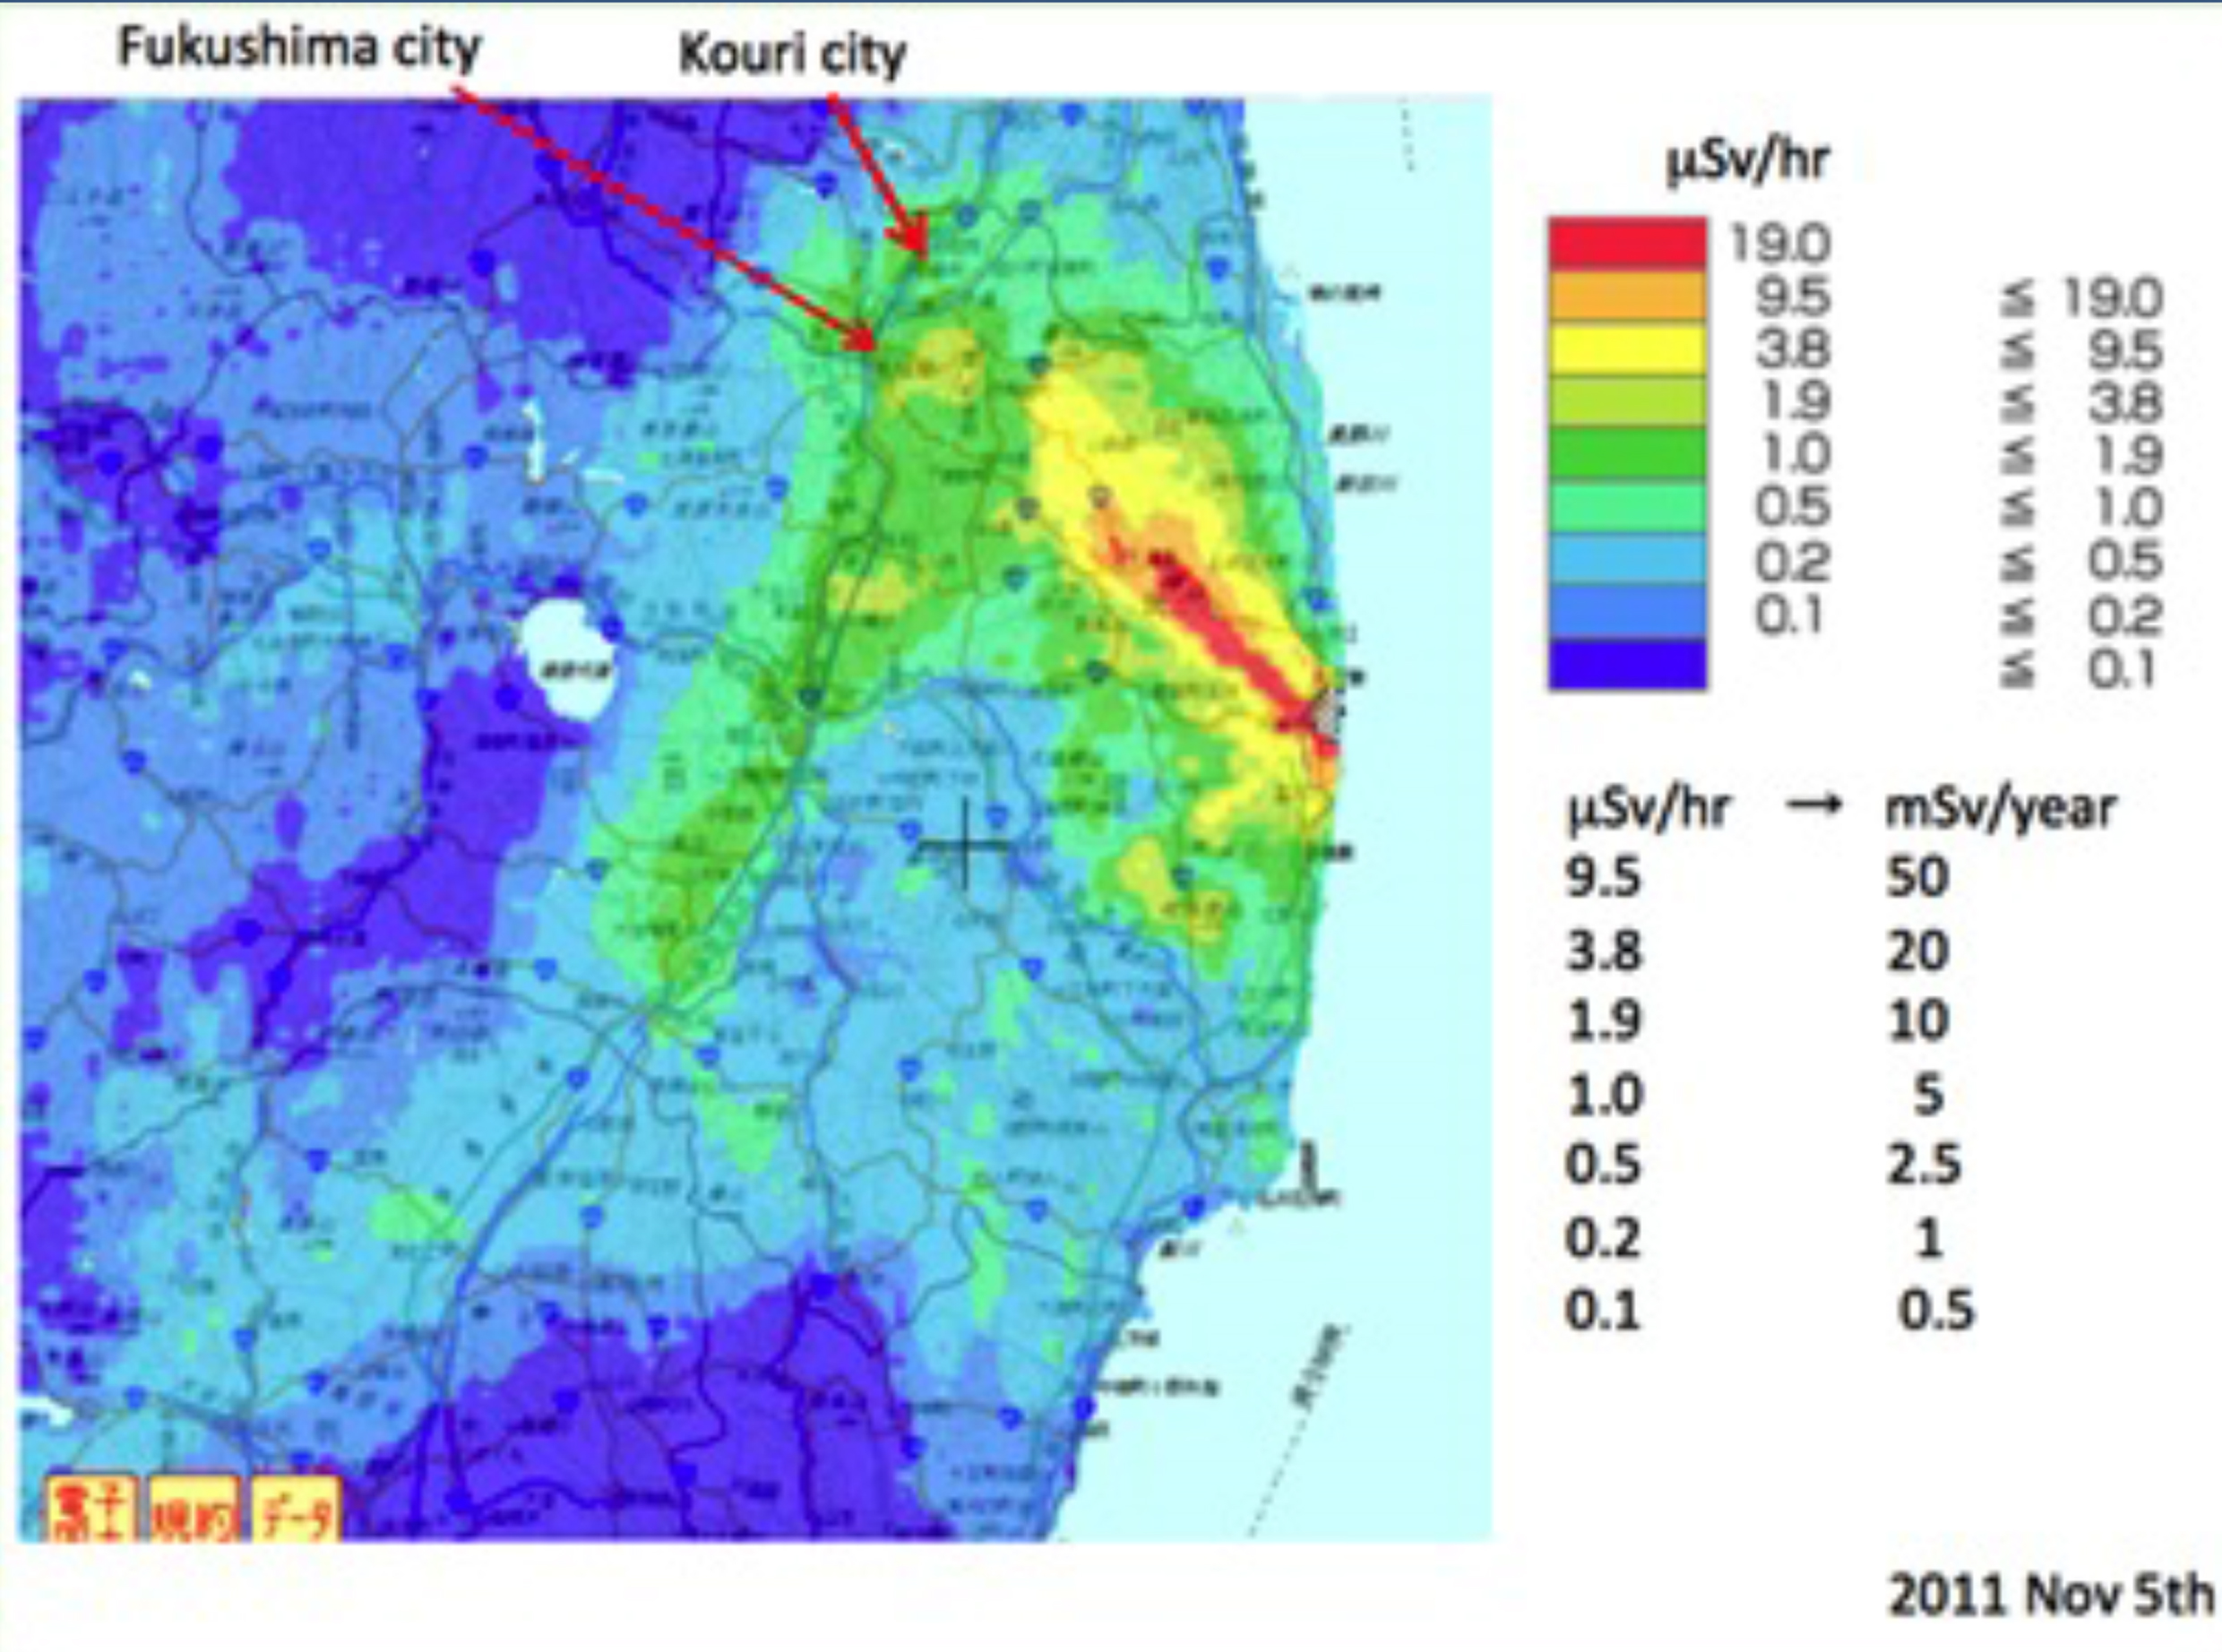
\includegraphics[width=1\textwidth]{figures/fukushima_disaster.jpg}
			%\caption{Fukushima Disaster (2011)}
			%\label{fig:fukushima_disaster}
		\end{figure}
		Coupled architecture
		\begin{itemize}
			\item Maintenance of relative positions important (e.g asdf) 
			\item inter-agent distances are low
			\item High disturbances
		\end{itemize}
	\end{minipage} 
	\begin{itemize}
		\item Combination of the two		
	\end{itemize}
\end{frame}
%%%%%%%%%%%%%%%%%%%%%%%%%%%%%%%%%%%%%%%%%%%%%%%%%%%%%%%%%%%%%%%%%%%%%
%%%%%%%%%%%%%%%%%%%%%%%%%%%%%%%%%%%%%%%%%%%%%%%%%%%%%%%%%%%%%%%%%%%%%
\begin{frame}{Coupled architecture: Consensus/ Formation control}	
	\begin{figure}
		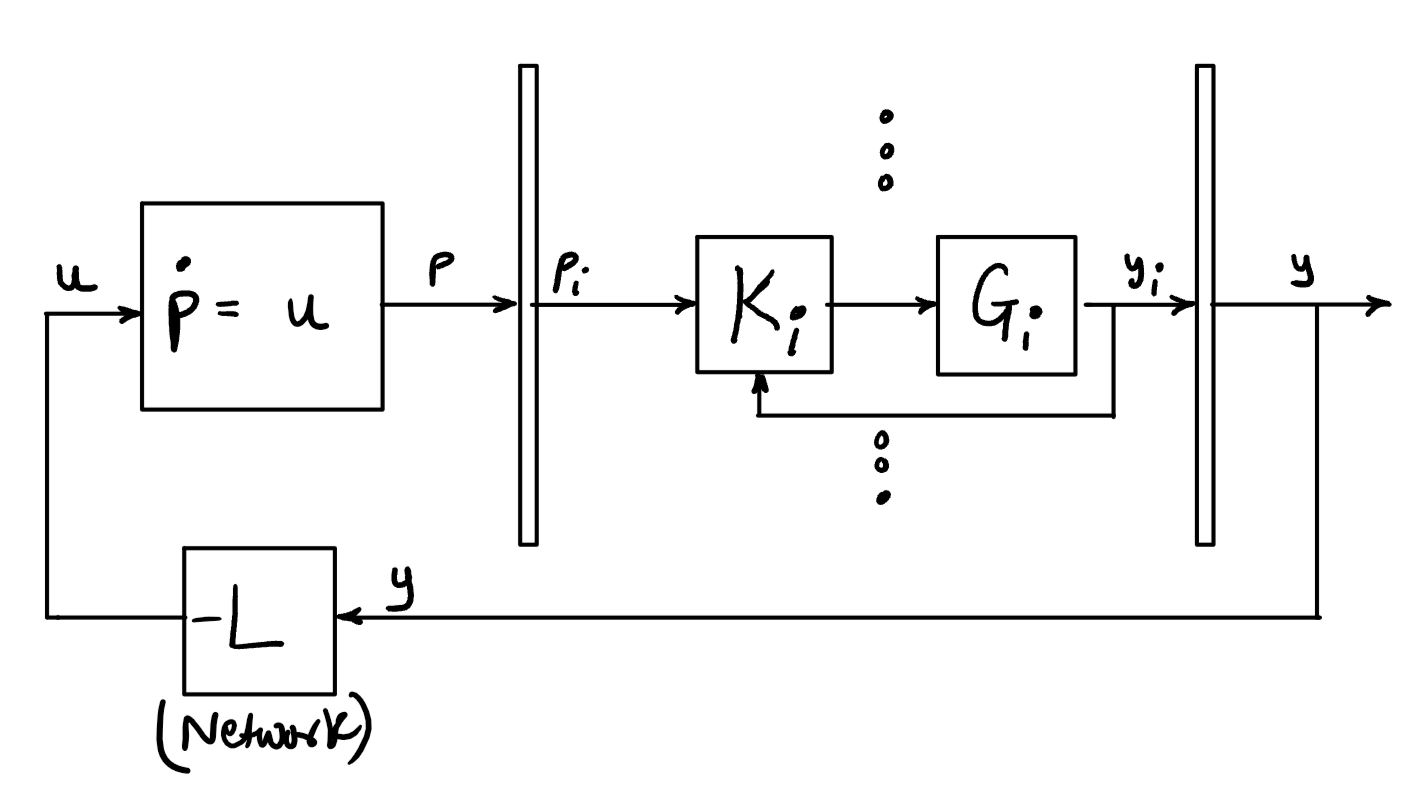
\includegraphics[scale=0.35]{figures/Coupled_consensus.jpg}	
		\label{fig:Coupled}
	\end{figure}
	\begin{itemize}
		\item Some related work
		\begin{itemize}
			\item Fixed Laplacian and LTI agents \footnote{Fax and Murray, 2004} -> Modal decomposition
			\item Fixed and uncertain Laplacian and LPV agents \footnote{Popov, 2009, Eichler and Hoffmann,2014} -> Modal decomposition 
			\item Flocking with a fixed Laplacian \footnote{B.Francis, 2016}	
			\item Interconnections of dissipative systems \footnote{M. Spong, 2006}		
		\end{itemize}
	\end{itemize}
\end{frame}
%%%%%%%%%%%%%%%%%%%%%%%%%%%%%%%%%%%%%%%%%%%%%%%%%%%%%%%%%%%%%%%%%%%%%
%%%%%%%%%%%%%%%%%%%%%%%%%%%%%%%%%%%%%%%%%%%%%%%%%%%%%%%%%%%%%%%%%%%%%
\begin{frame}{Coupled architecture: Flocking}	
	\begin{figure}
		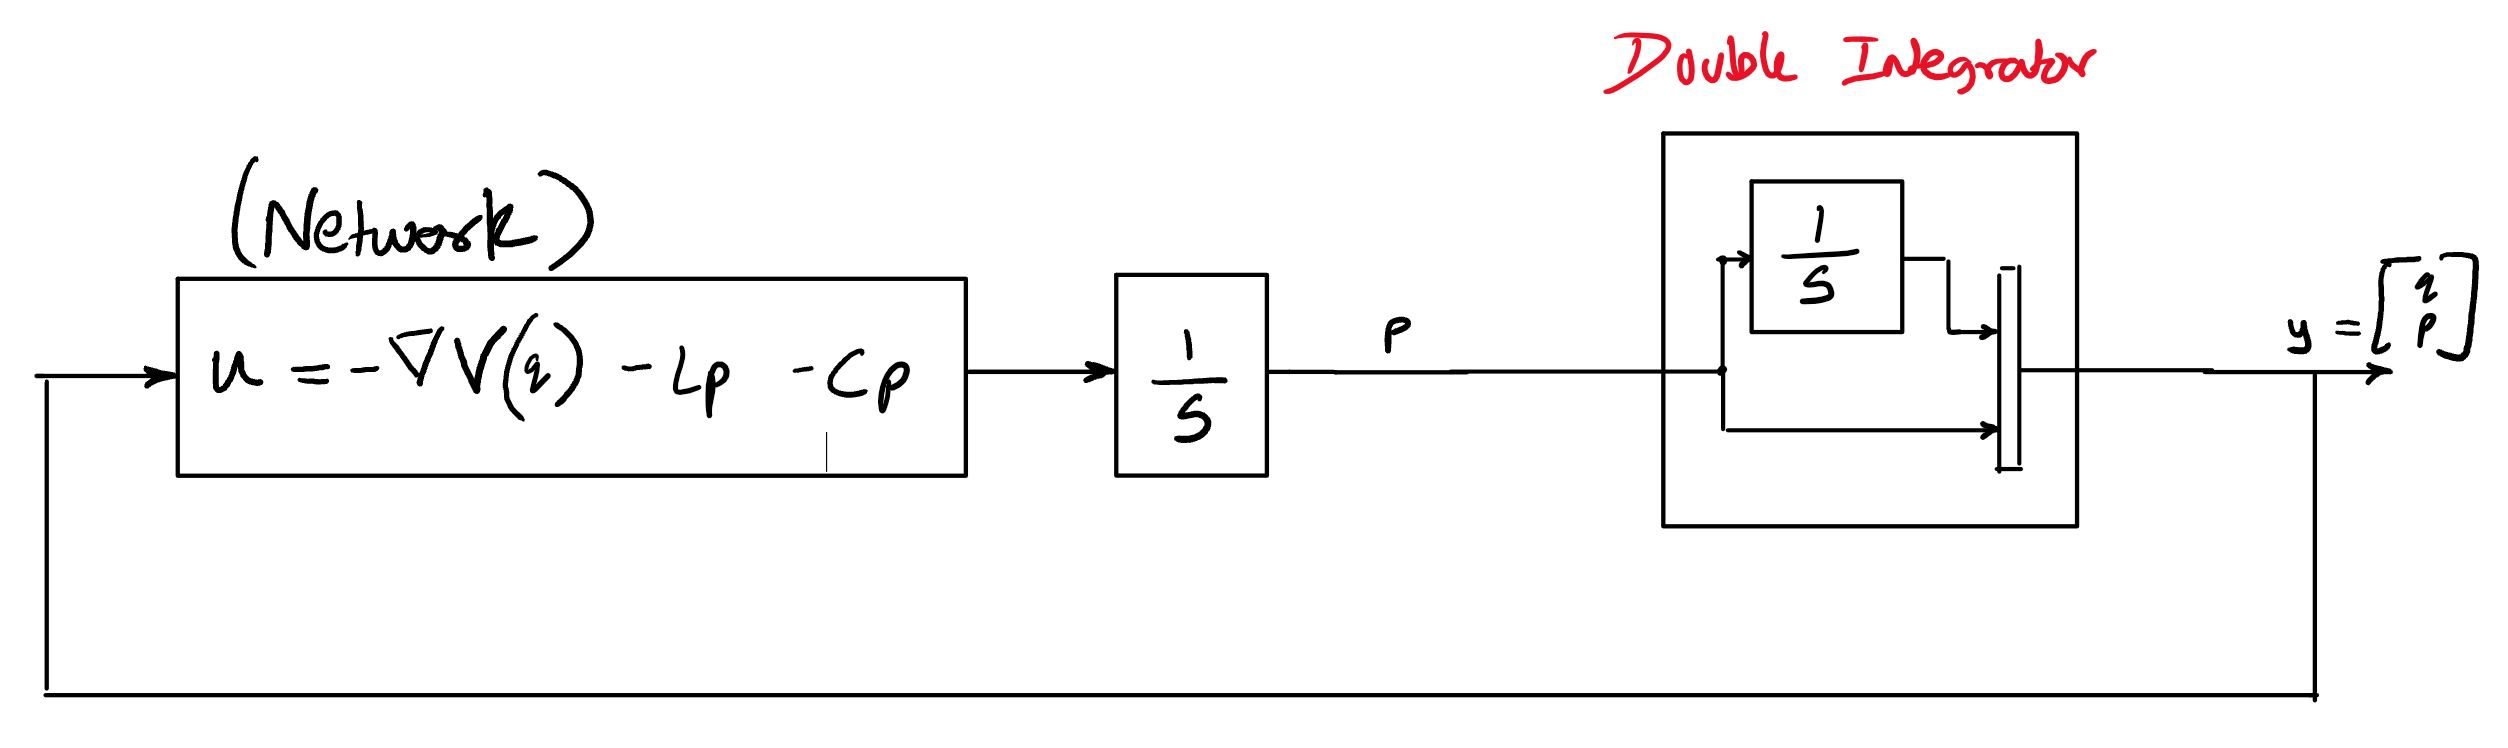
\includegraphics[scale=0.35]{figures/Coupled_flocking_double_integrators.jpg}	
		\label{fig:Coupled}
	\end{figure}
	\begin{itemize}
		\item Flocking of double integraor agents \footnote{Olfati Saber,2006}
		\item Stability analysis via LaSalle
	\end{itemize}
\end{frame}
%%%%%%%%%%%%%%%%%%%%%%%%%%%%%%%%%%%%%%%%%%%%%%%%%%%%%%%%%%%%%%%%%%%%%
%%%%%%%%%%%%%%%%%%%%%%%%%%%%%%%%%%%%%%%%%%%%%%%%%%%%%%%%%%%%%%%%%%%%%
\begin{frame}{Coupled architecture: Flocking}	
	\begin{figure}
		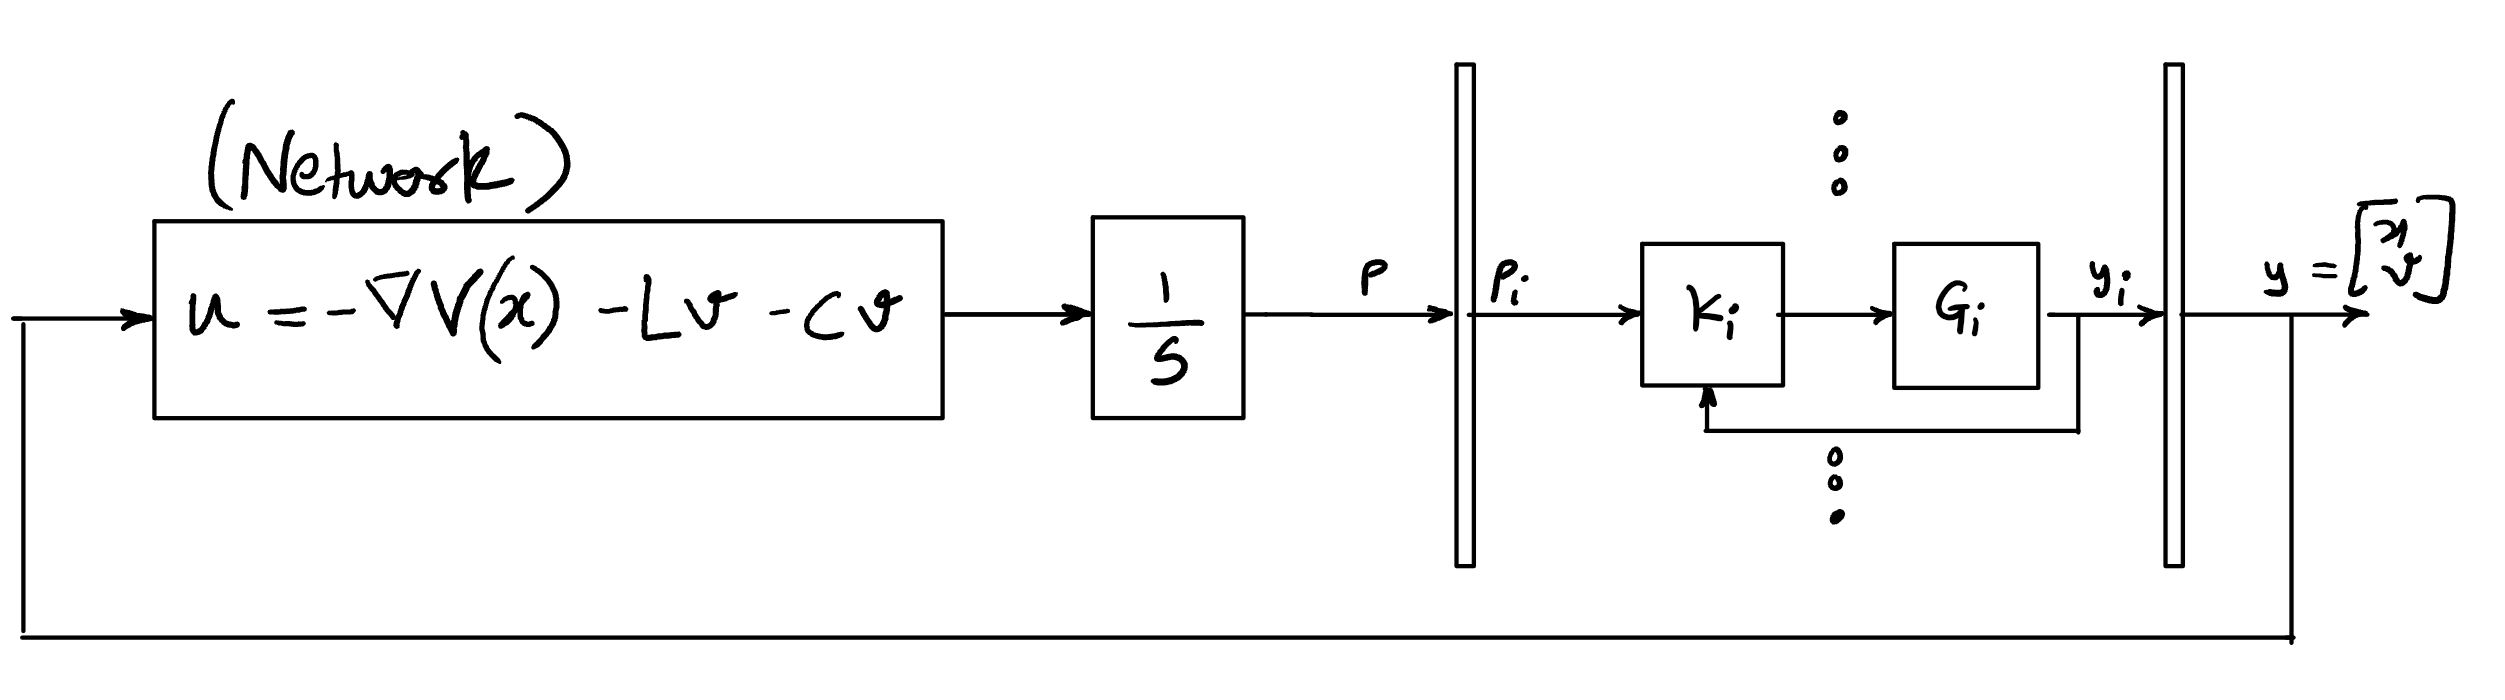
\includegraphics[scale=0.35]{figures/Coupled_flocking_quads.jpg}	
		\label{fig:Coupled}
	\end{figure}
	\begin{itemize}
		\item Flocking of quadrotors agents \footnote{Francis, 2016} but with fixed Laplacians
		\item Our experiments show that Quadrotors can be made to act like double integrators by well-tuned velocity controllers
	\end{itemize}
\end{frame}
%%%%%%%%%%%%%%%%%%%%%%%%%%%%%%%%%%%%%%%%%%%%%%%%%%%%%%%%%%%%%%%%%%%%%
%%%%%%%%%%%%%%%%%%%%%%%%%%%%%%%%%%%%%%%%%%%%%%%%%%%%%%%%%%%%%%%%%%%%%
\begin{frame}{Coupled architecture: Flocking and source-seeking \footnote{Datar, Paulsen, Werner, 2020}}
	\begin{figure}
		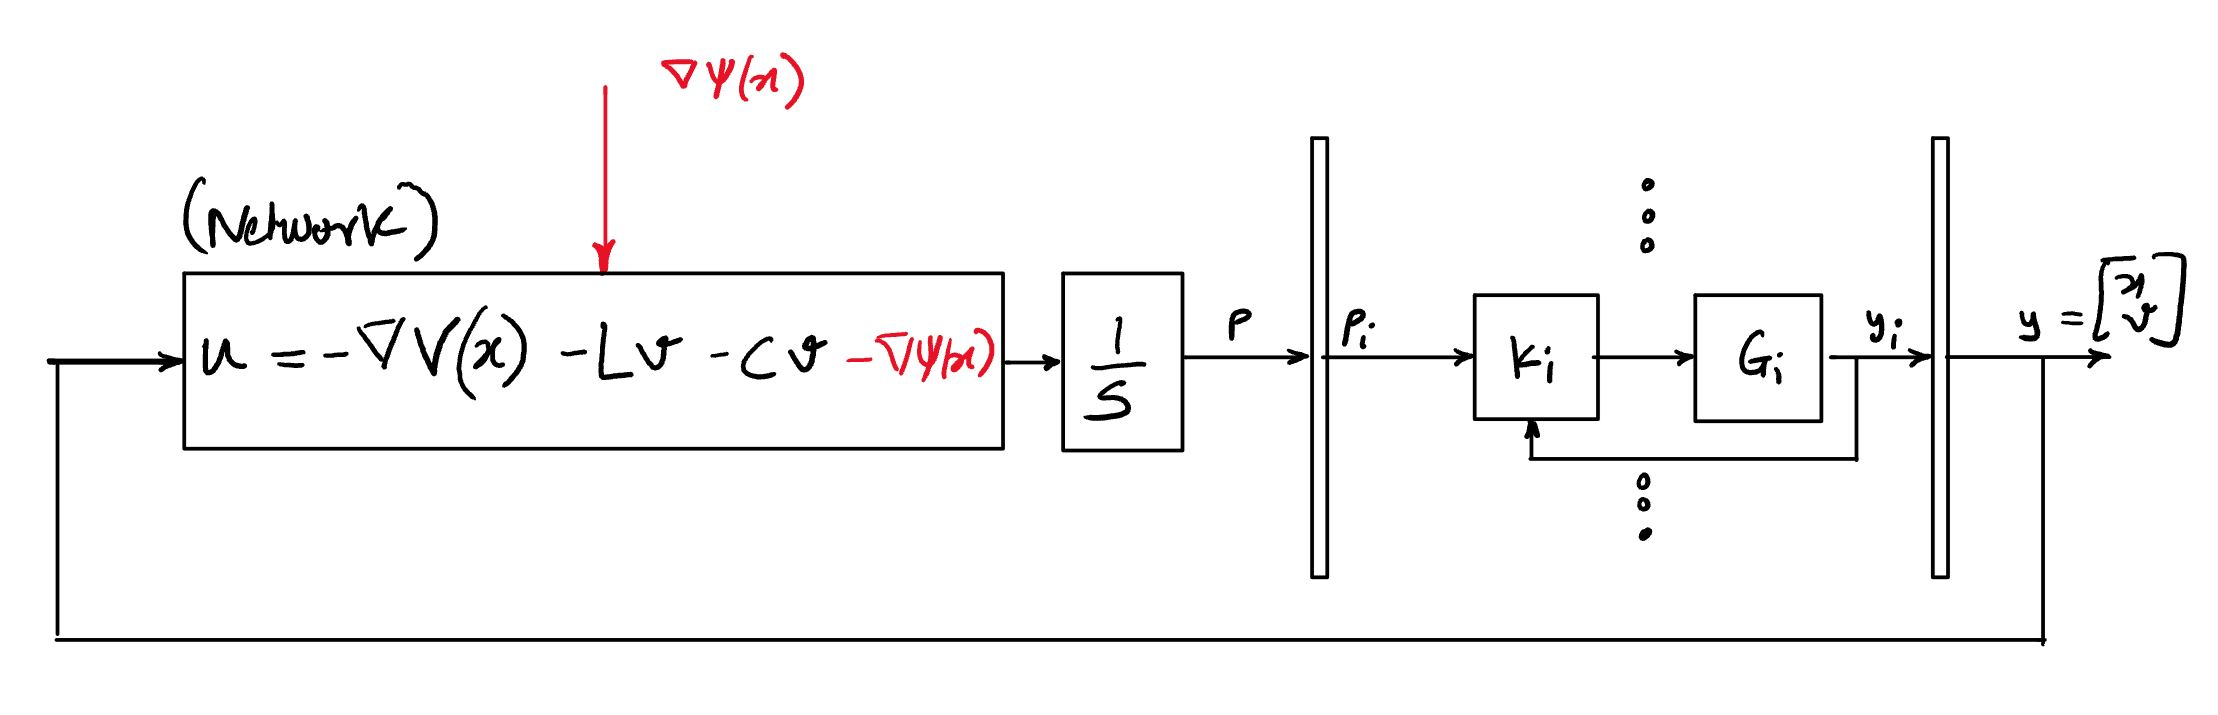
\includegraphics[scale=0.35]{figures/Coupled_flocking_quads_source_seek.jpg}	
		\label{fig:Coupled}
	\end{figure}	
	\begin{itemize}
		\item Forcing dynamics due to a scalar field
		\item Convergence analysis(Asymptotic stability) for double integrator agents
		\item Experiments by designing good local velocity controllers
	\end{itemize}
\end{frame}
%%%%%%%%%%%%%%%%%%%%%%%%%%%%%%%%%%%%%%%%%%%%%%%%%%%%%%%%%%%%%%%%%%%%%
%%%%%%%%%%%%%%%%%%%%%%%%%%%%%%%%%%%%%%%%%%%%%%%%%%%%%%%%%%%%%%%%%%%%%
\begin{frame}{Coupled architecture: Flocking and source-seeking with non-linear agents \footnote{Atallah, Datar, Werner, 2020}}	
	\begin{figure}
		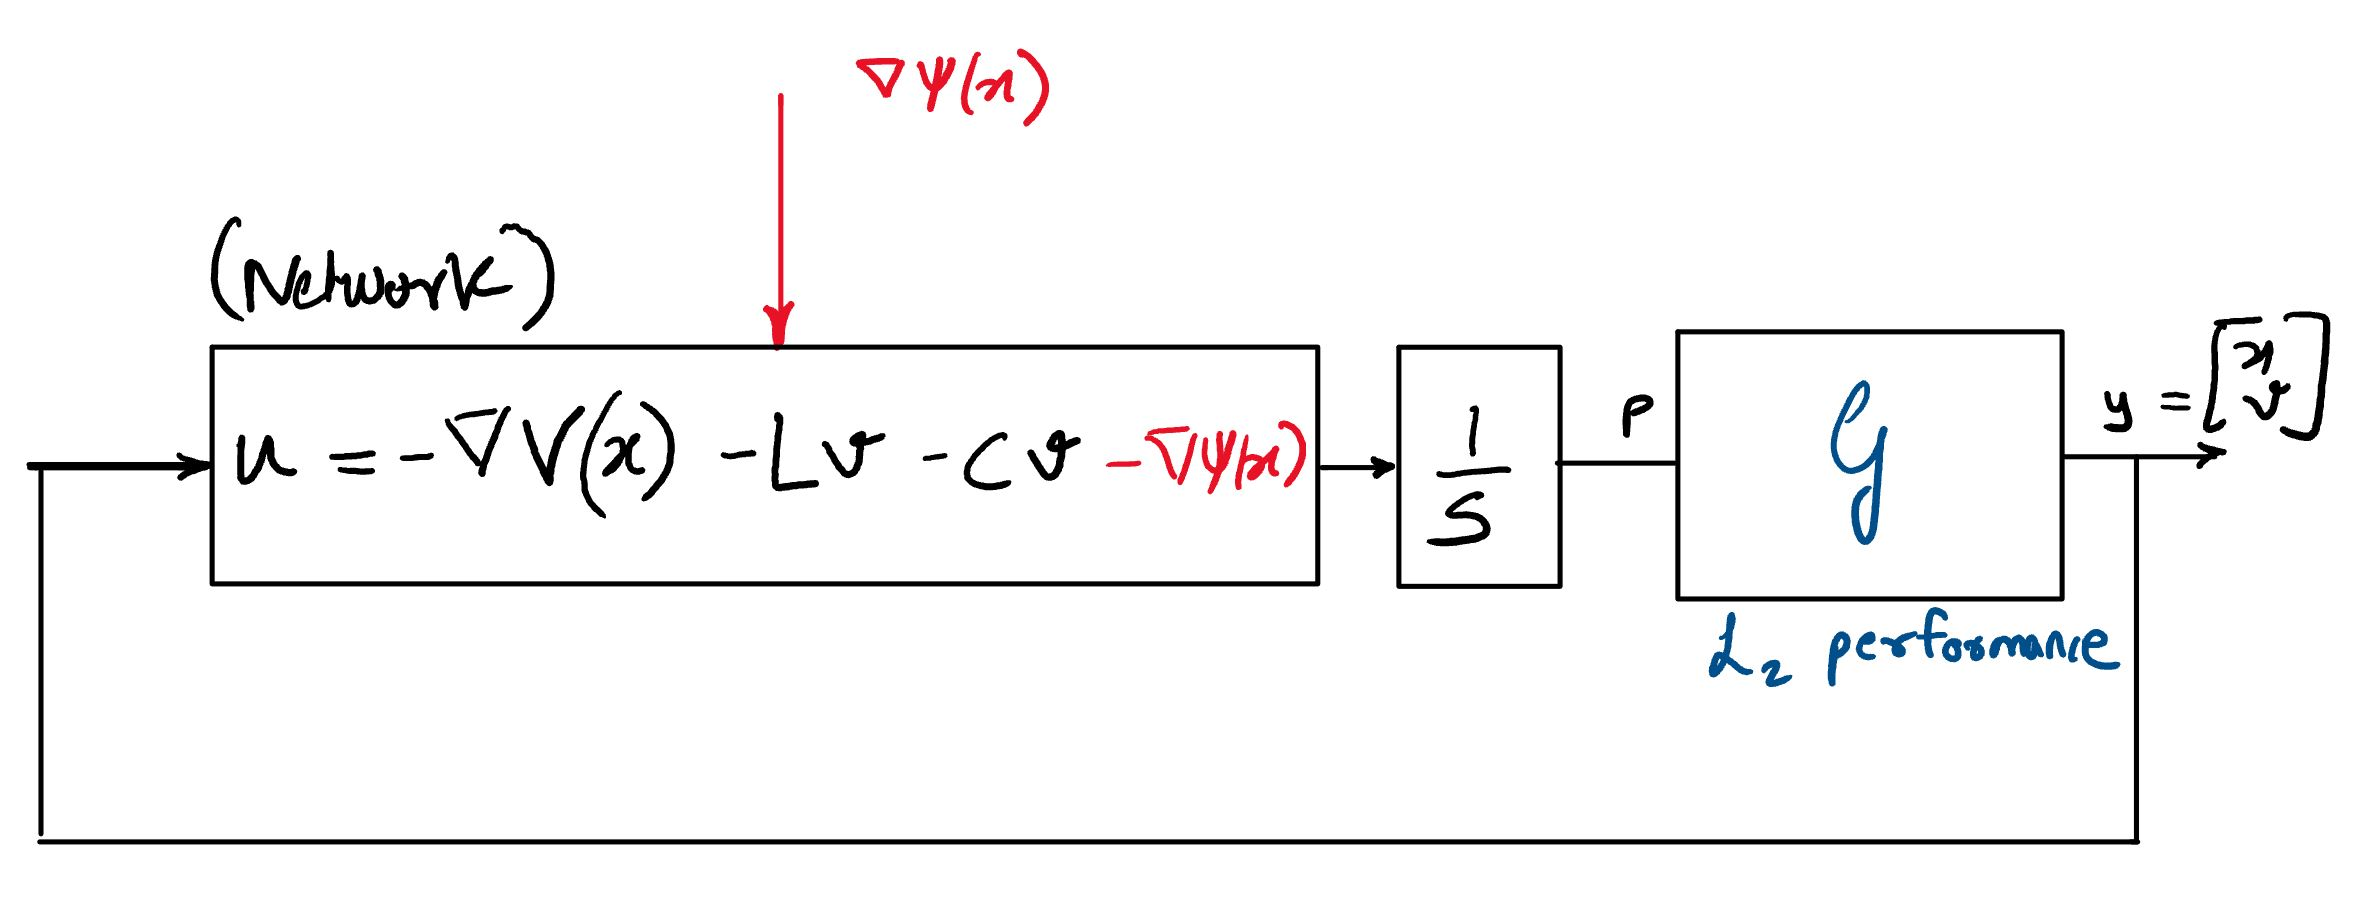
\includegraphics[scale=0.35]{figures/Coupled_flocking_gen_non_lin.JPG}	
		\label{fig:Coupled}
	\end{figure}
	\begin{itemize}
		\item From double integrators -> non-linear (LPV) agents
		\item Stability isL(not asymptotic) 
	\end{itemize}
\end{frame}
%%%%%%%%%%%%%%%%%%%%%%%%%%%%%%%%%%%%%%%%%%%%%%%%%%%%%%%%%%%%%%%%%%%%%
%%%%%%%%%%%%%%%%%%%%%%%%%%%%%%%%%%%%%%%%%%%%%%%%%%%%%%%%%%%%%%%%%%%%%
\begin{frame}{Coupled architecture: Some speculative ideas and open questions}	
	\begin{figure}
		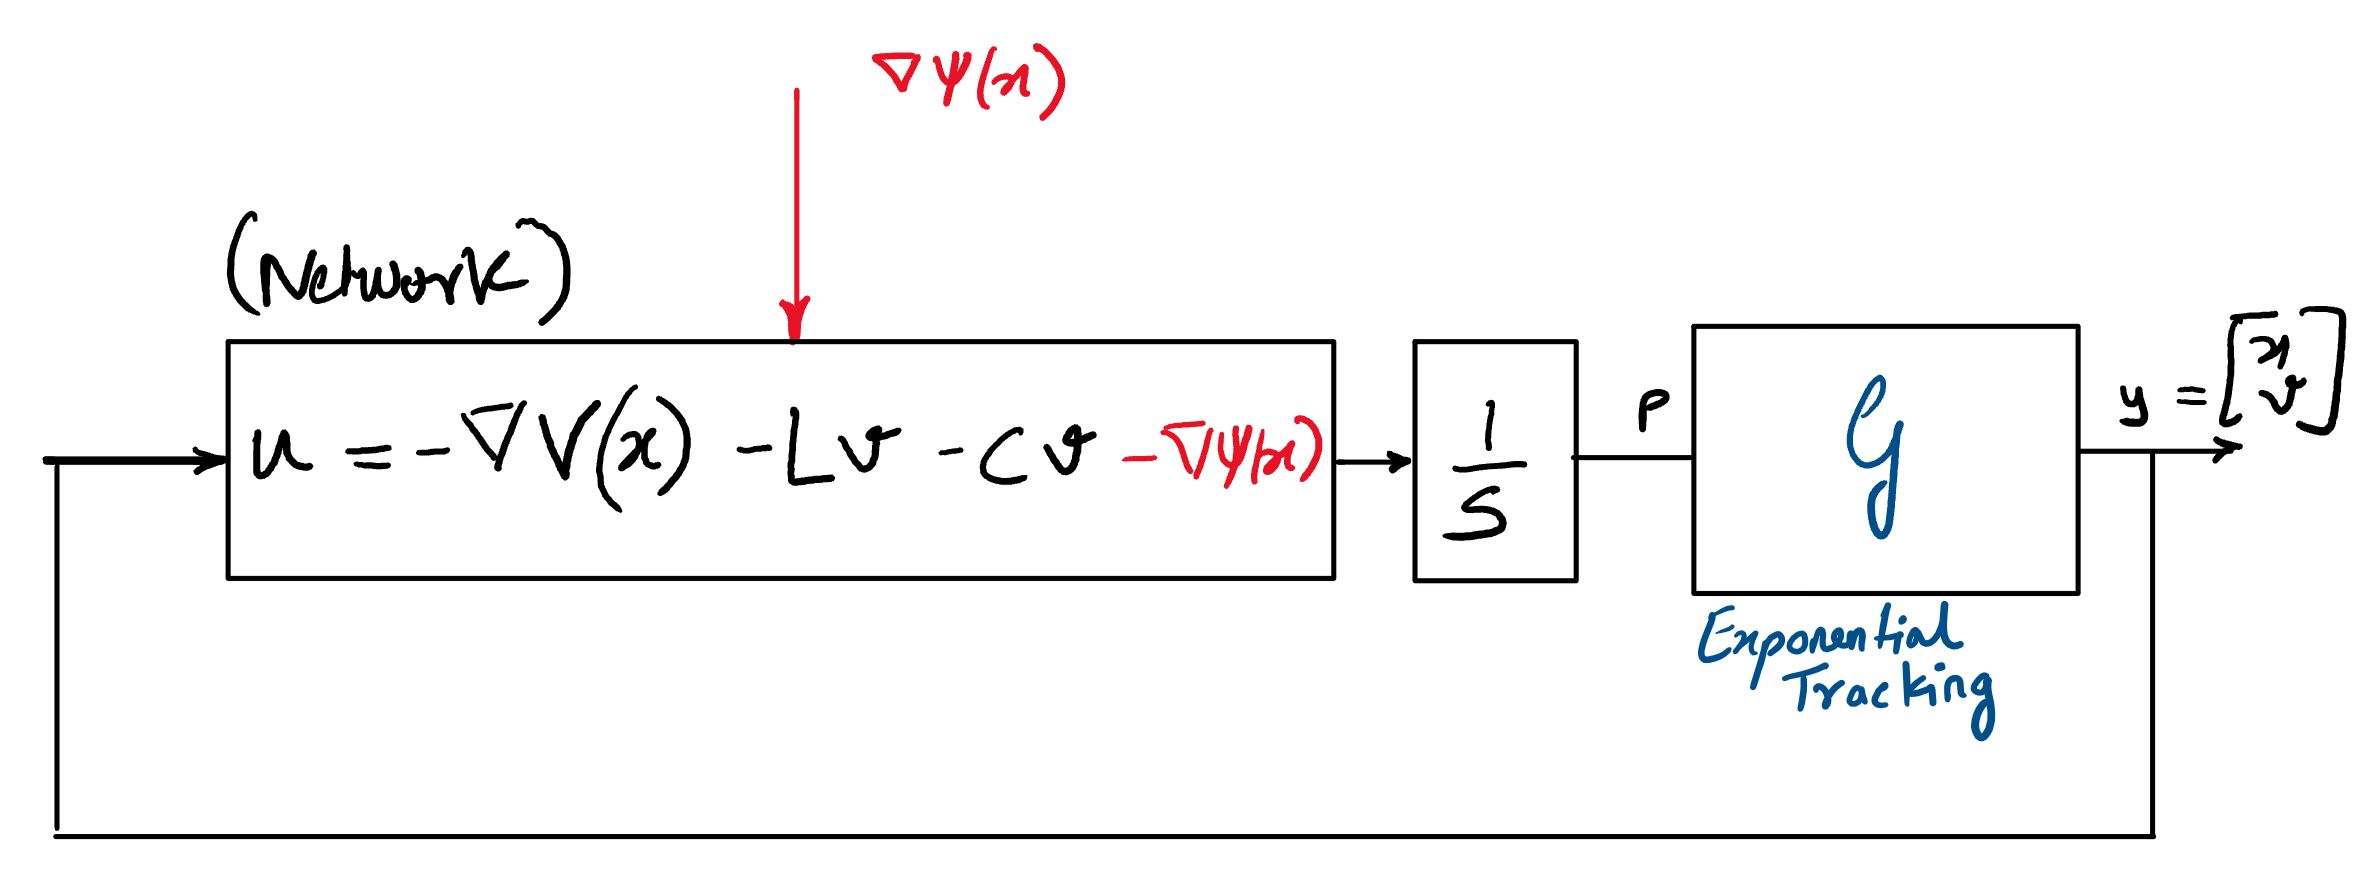
\includegraphics[scale=0.35]{figures/Coupled_flocking_gen_IQC.JPG}	
		\label{fig:Coupled}
	\end{figure}
	\begin{itemize}
		\item Use IQCs to obtain exponential convergence rates\footnote{Boczr,Recht,Lessard,Packard,2017} of local closed loops and use  singular perturbation argument such as in \footnote{Mesbahi and others,2018} 
	\end{itemize}
\end{frame}
%%%%%%%%%%%%%%%%%%%%%%%%%%%%%%%%%%%%%%%%%%%%%%%%%%%%%%%%%%%%%%%%%%%%%
%%%%%%%%%%%%%%%%%%%%%%%%%%%%%%%%%%%%%%%%%%%%%%%%%%%%%%%%%%%%%%%%%%%%%
\begin{frame}{Decoupled architecture: Consensus/ Formation control}
	\begin{figure}
		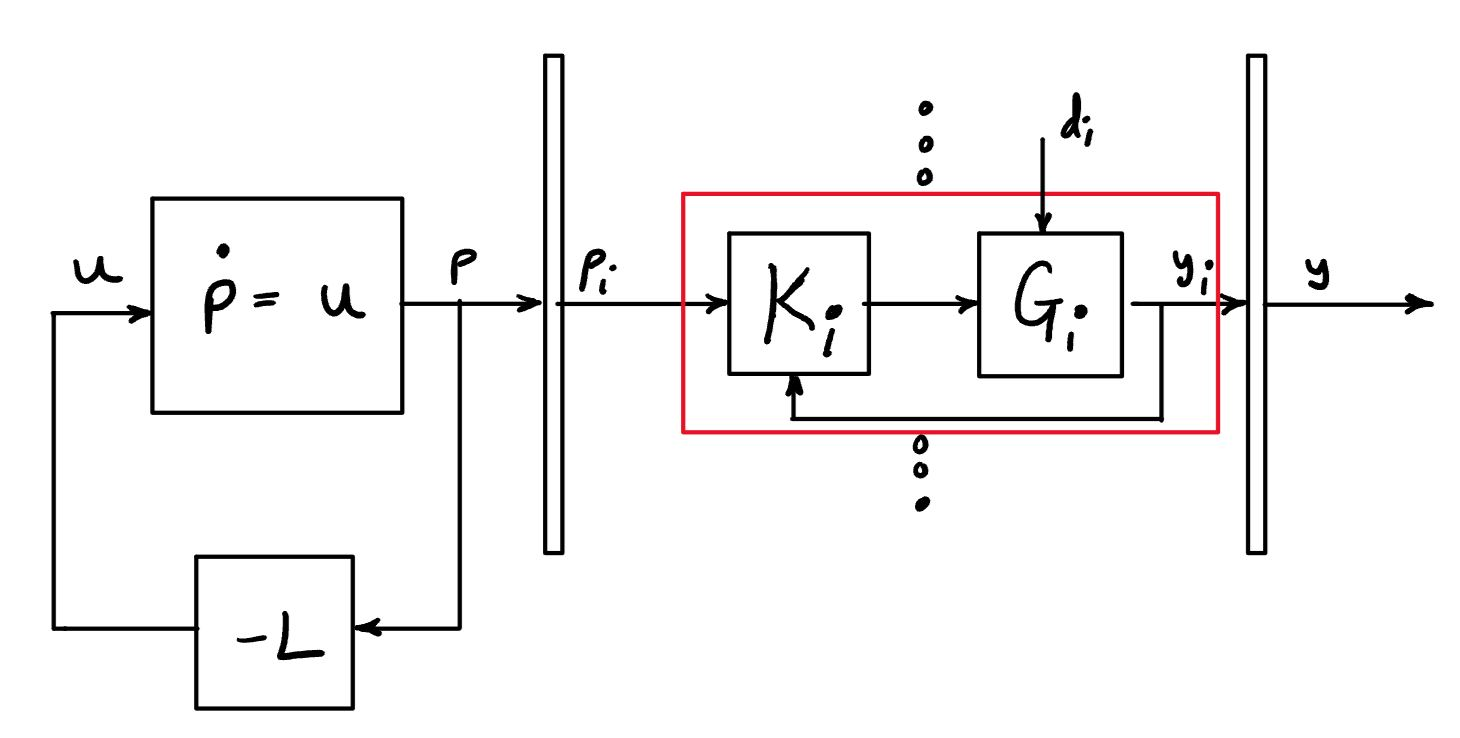
\includegraphics[scale=0.35]{figures/decoupled_consensus.JPG}	
		\label{fig:Coupled}
	\end{figure}
	\begin{itemize}
		\item Some related work
		\begin{itemize}
			\item Idea of wrapping local controllers around first order dynamics \footnote{Egerstedt and Cortes,2017}
			\item Combine a cooperation module with consensus moduke \footnote{Chen and Ren, 2019}
			\item Discrete-time Information flow filter \footnote{Fax and Murray, 2004}
		\end{itemize}
	\end{itemize}
\end{frame}
%%%%%%%%%%%%%%%%%%%%%%%%%%%%%%%%%%%%%%%%%%%%%%%%%%%%%%%%%%%%%%%%%%%%%
%%%%%%%%%%%%%%%%%%%%%%%%%%%%%%%%%%%%%%%%%%%%%%%%%%%%%%%%%%%%%%%%%%%%%
\begin{frame}{Decoupled architecture: Formation forming}	
		\begin{figure}
		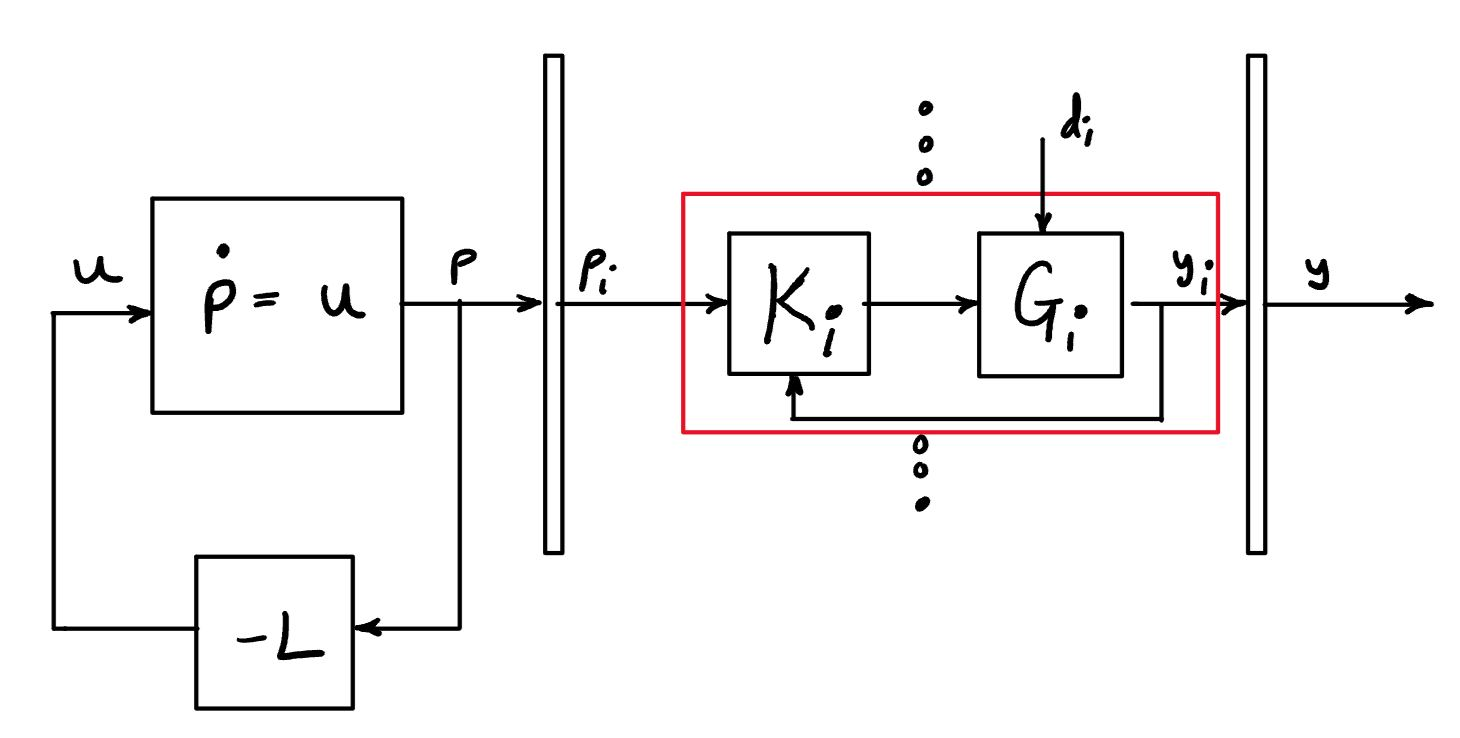
\includegraphics[scale=0.35]{figures/decoupled_consensus.JPG}	
		\label{fig:Coupled}
	\end{figure}
	\begin{itemize}
		\item Gen H2 norm\footnote{Hespe, 2020}
		\item Positive systems theory in the network loop\footnote{Datar, 2020 (Submitted)}
		\item Crazyflie experiments \footnote{M. Thesis, Paulsen,2019}
	\end{itemize}
\end{frame}
%%%%%%%%%%%%%%%%%%%%%%%%%%%%%%%%%%%%%%%%%%%%%%%%%%%%%%%%%%%%%%%%%%%%%
%%%%%%%%%%%%%%%%%%%%%%%%%%%%%%%%%%%%%%%%%%%%%%%%%%%%%%%%%%%%%%%%%%%%%
\begin{frame}{Decoupled architecture: Non-ideal networks}
	\begin{figure}
		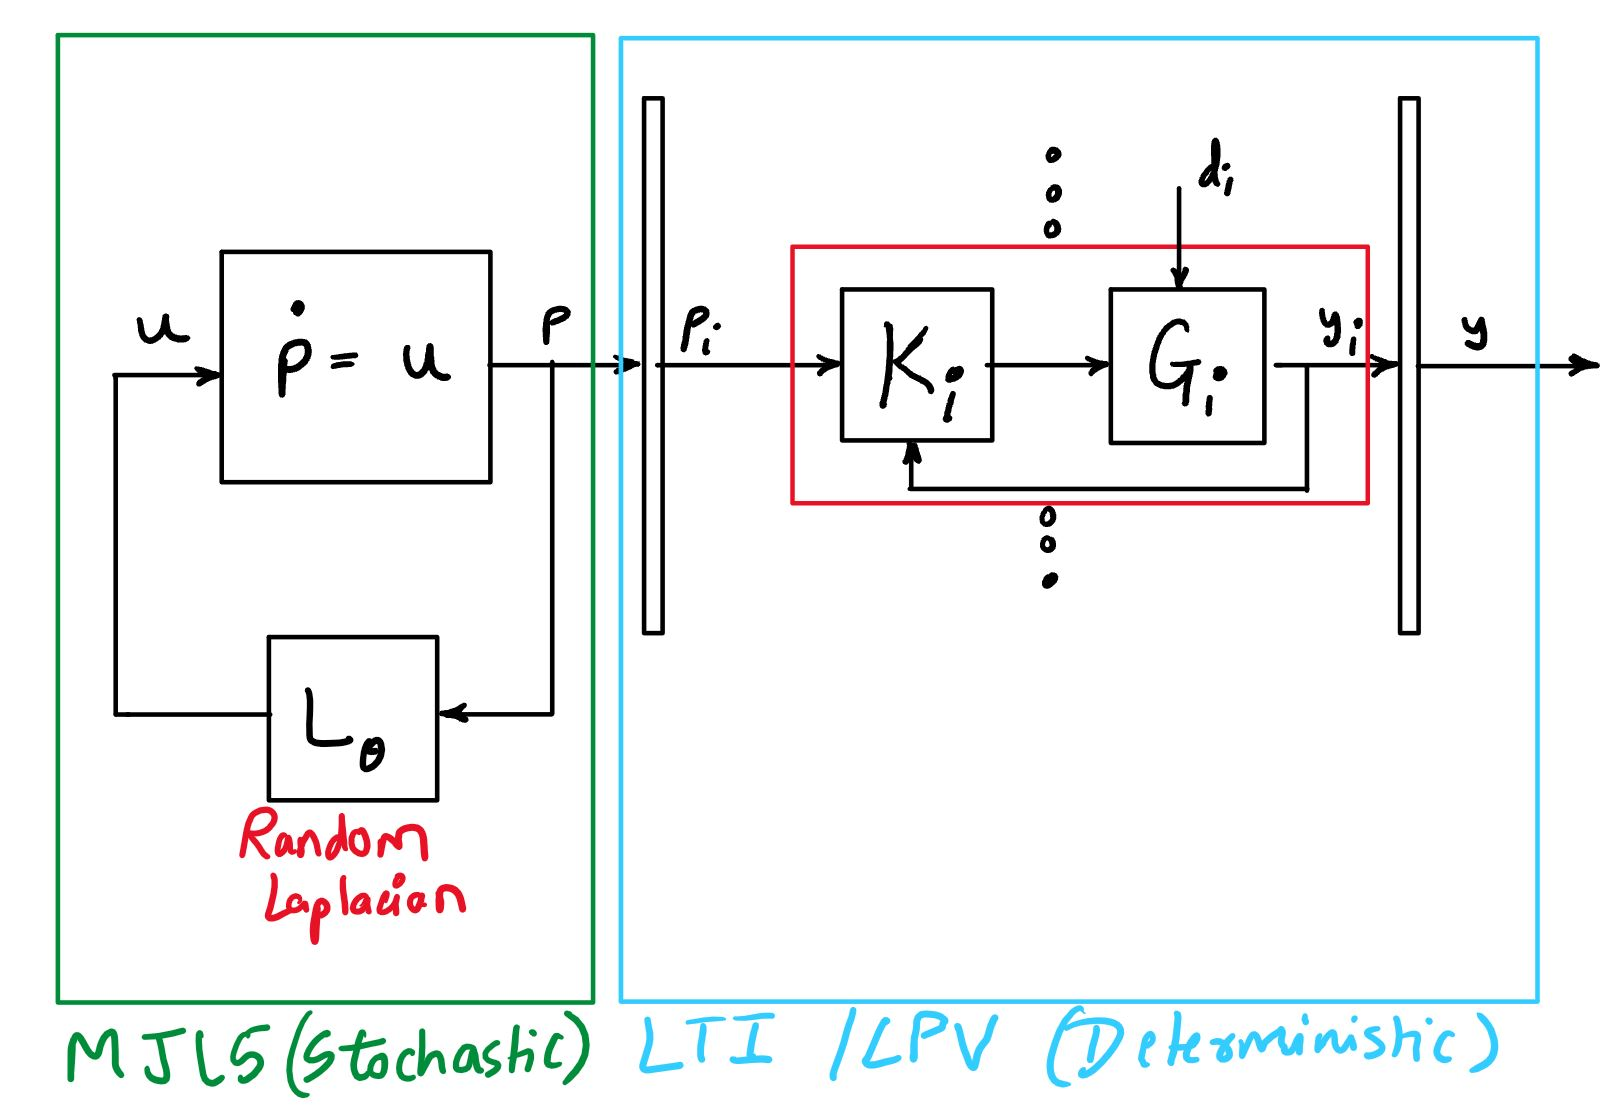
\includegraphics[scale=0.35]{figures/decoupled_stoch_deterministic.JPG}	
		\label{fig:Coupled}
	\end{figure}
	\begin{itemize}
		\item Model the Information flow dynamics as a Markovian Jump Linear System(MJLS)
		\item r2 or w2 measures (Daniel will talk more about this)
		\item IQC analysis of consensus Dynamics \footnote{Rantzer, 2016} -> Scalable condition
	\end{itemize}
\end{frame}
%%%%%%%%%%%%%%%%%%%%%%%%%%%%%%%%%%%%%%%%%%%%%%%%%%%%%%%%%%%%%%%%%%%%%
\begin{frame}{Conclusions}	
	\begin{itemize}
		\item asdf
	\end{itemize}
\end{frame}
%%%%%%%%%%%%%%%%%%%%%%%%%%%%%%%%%%%%%%%%%%%%%%%%%%%%%%%%%%%%%%%%%%%%%
\begin{frame}{}
\begin{center}
    \huge{Thank you}
\end{center}
\end{frame}
%%%%%%%%%%%%%%%%%%%%%%%%%%%%%%%%%%%%%%%%%%%%%%%%%%%%%%%%%%%%%%%%%%%%%
%\section{Flocking algorithms to address the source-seeking problem}
\subsection{Problem}
%%%%%%%%%%%%%%%%%%%%%%%%%%%%%%%%%%%%%%%%%%%%%%%%%%%%%%%%%%%%%%%%%%%%%
\begin{frame}{Source seeking problem: Abstraction}
	
\begin{itemize}
	\item A group of $N$ agents (e.g underwater robots) are deployed in the region of interest
	\item Each agent has the following properties:
	    \begin{itemize}
	        \item Absolute position measurement (e.g GPS)\footnote{This assumption can be removed as long there is relative displacement measurement}
	        \item Communication with agents within a fixed distance
	        \item Concentration measurement sensor
	        \item Computation capabilities 
	    \end{itemize}
	\item \textbf{Problem:} Design distributed control algorithms that cause the agents to flock towards the source (location with the highest concentration) in a cooperative manner.
\end{itemize}
\end{frame}
\subsection{Theory}
%%%%%%%%%%%%%%%%%%%%%%%%%%%%%%%%%%%%%%%%%%%%%%%%%%%%%%%%%%%%%%%%%%%%%
% \begin{frame}{Capabilities of a single agent (Robot)}
% \begin{itemize}
% 	\item Position information based on an indoor positioning system (can be relaxed to only distance measurements)
% 	\item Peer to peer communication and computation capabilites onboard
% 	\item Pretend to measure the strength of a virtual scalar field based on the current location
% \end{itemize}		
% \end{frame}
%%%%%%%%%%%%%%%%%%%%%%%%%%%%%%%%%%%%%%%%%%%%%%%%%%%%%%%%%%%%%%%%%%%%%
\begin{frame}{Source seeking problem as optimization}
\begin{itemize} 
	\item Look at the source seeking problem as a minimization problem
	\item Momentum methods\footnote{Polyak,1964} have been used in optimization to speed up or dampen the oscillations
	\item Naturally have momentum of the mobile robots   
	\item For theoretical analysis: Use continuous-time versions of optimization methods to study the assymptotic properties\footnote{Redont et al., 2002} 
\end{itemize}
\end{frame}
% %%%%%%%%%%%%%%%%%%%%%%%%%%%%%%%%%%%%%%%%%%%%%%%%%%%%%%%%%%%%%%%%%%%%%
% \begin{frame}{Continuous-time steepest descent with momentum}
% \begin{itemize}
% \item Consider the problem of minimizing a differentiable $f:\mathbb{R}^n\rightarrow \mathbb{R}$
% \pause
% \item The steepest descent iteration is
% \begin{equation}
% x_{k+1}=x_k - \alpha \nabla f(x_k)
% \end{equation}
% \pause
% \item The continuous-time version of the steepest descent dynamics 
% \begin{equation}
% \dot{x}= - \nabla f(x_k)
% \end{equation}
% \pause
% \item The continuous-time version of the steepest descent dynamics with momentum (also known as the heavy ball method with friction) 
% \begin{equation}
% m\ddot{x}+ \dot{x}= - \nabla f(x_k)
% \end{equation}
% \end{itemize}
% \end{frame}
%%%%%%%%%%%%%%%%%%%%%%%%%%%%%%%%%%%%%%%%%%%%%%%%%%%%%%%%%%%%%%%%%%%%%
\begin{frame}{Continuous-time Newton method with momentum}
\begin{itemize}
	\item Consider the problem of minimizing a twice-differentiable, strongly convex $f:\mathbb{R}^n\rightarrow \mathbb{R}$
	\pause
	\item The Newton iteration is
	\begin{equation}
	x_{k+1}=x_k - \alpha\nabla^2f(x_k)^{-1} \nabla f(x_k)
	\end{equation}
	\pause
	\item The continuous-time version of these dynamics can be represented as
	\begin{equation}
	\nabla^2f(x_k)\dot{x}= - \nabla f(x_k)
	\end{equation}
	\pause
	\item Adding momentum to these dynamics gives  
	\begin{equation}
	m\ddot{x}+ \nabla^2f(x_k)\dot{x}= - \nabla f(x_k)
	\end{equation}
\end{itemize}
\pause
Defining the velocity variable $v$, the dyanmics can be written as 
\begin{equation} \label{eqn: second_order_newton_cont_time}
\begin{split}
\Dot{x}&=v\\
\Dot{v}&=-k_1\nabla^2 f(x) v -k_2 \nabla f(x), 
\end{split}
\end{equation}
\end{frame}
%%%%%%%%%%%%%%%%%%%%%%%%%%%%%%%%%%%%%%%%%%%%%%%%%%%%%%%%%%%%%%%%%%%%%
\begin{frame}{Flocking and schooling in nature}

\begin{minipage}{0.45\textwidth}	
	%\hspace{0.4cm}	
	\begin{figure}
		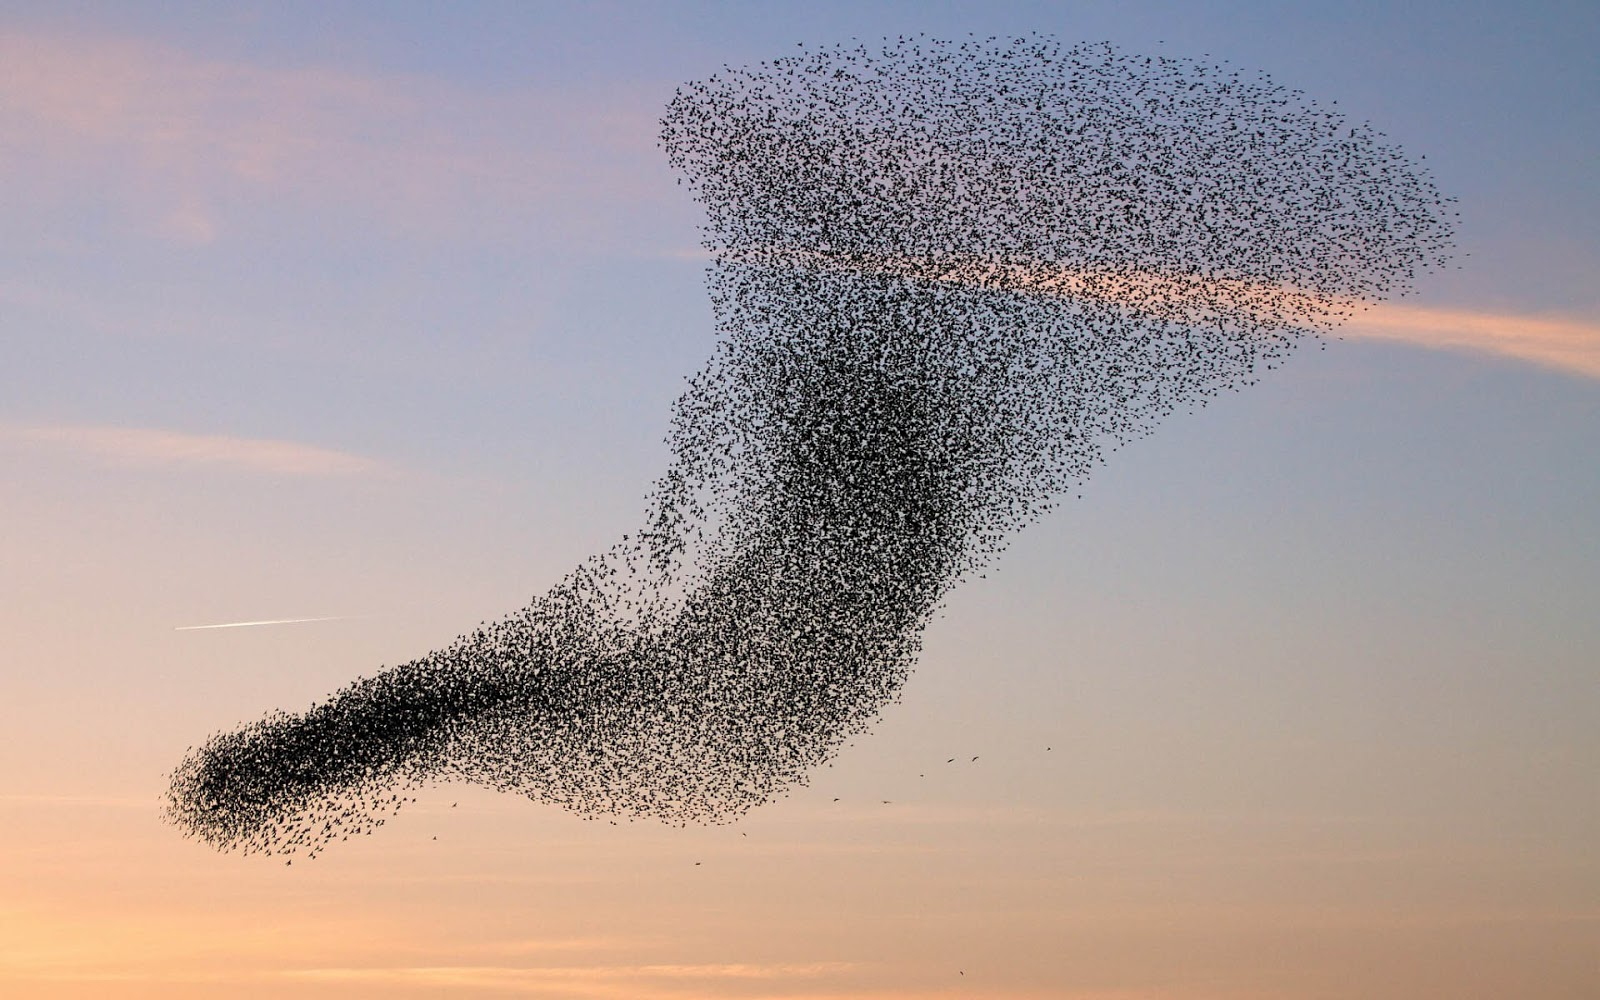
\includegraphics[width=\textwidth]{figures/flock_of_birds.jpg}
		%\caption{Fukushima Disaster}
		%\label{fig:flock_of_birds}
	\end{figure}
\end{minipage}
\hspace{0.05cm}
\begin{minipage}{0.45\textwidth}	
	\begin{figure}
		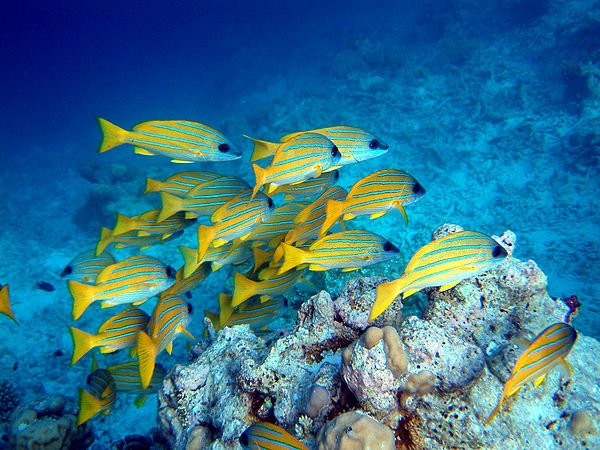
\includegraphics[width=\textwidth]{figures/schooling_fish.jpg}
		%\caption{Oil Spills}
		%\label{fig:schools_of_fish}
	\end{figure}
\end{minipage}
\begin{itemize}	
	\item The precise rules that these animals use are not known
	\item Particle-based flocking seems to be an effective approach to model such behavior
	\item In 1987, Reynold was working on animating flocking behavior where he proposed three rule
	\begin{itemize}
		\item Cohesion: Attempt to stay close to nearby neighbors
		\item Separation: Avoid collisions with nearby flockmates
		\item Alignment: attempt to match velocities with nearby flockmates
	\end{itemize}
\end{itemize}
\end{frame}
%%%%%%%%%%%%%%%%%%%%%%%%%%%%%%%%%%%%%%%%%%%%%%%%%%%%%%%%%%%%%%%%%%%%%
\begin{frame}{Flocking dynamics}
\begin{itemize}
	\item Every particle interacts with every other particle based on an interaction field $V$ which depends only on the distance between them
	\item An example of a potential field is the gravitational field $V(z)=\frac{mMG}{||z||}$
	\item Flocking dynamics\footnote{Olfati-Saber, 2004}:
	\begin{equation*}
	\begin{split}
	\Dot{q}&=p\\
	\Dot{p}&=-\nabla V(q)-\hat{L}(q)p -cp 
	\end{split}
	\end{equation*}
\end{itemize}
\end{frame}
%%%%%%%%%%%%%%%%%%%%%%%%%%%%%%%%%%%%%%%%%%%%%%%%%%%%%%%%%%%%%%%%%%%%%
\begin{frame}{Flocking towards the source}
\begin{itemize}
\item Consider now an underlying source field $\psi:\mathbf{R}^m \xrightarrow{} \mathbf{R}$ which is smooth enough and convex.
\item Add a forcing term to the flocking dynamics motivated from the discussion on optimization
\item Flocking dynamics with source-seeking:
\begin{equation*}
\begin{split}
\Dot{q}&=p\\
\Dot{p}&=-\nabla V(q)-\hat{L}(q)p -cp\textcolor{red}{-k_1\nabla^2 \Psi(q) p -k_2 \nabla \Psi(q)}
\end{split}
\end{equation*}
\end{itemize}
\end{frame}
%%%%%%%%%%%%%%%%%%%%%%%%%%%%%%%%%%%%%%%%%%%%%%%%%%%%%%%%%%%%%%%%%%%%%
\begin{frame}{Stability(Convergence) Analysis}
	Flocking dynamics with source-seeking:
	\begin{equation*}
	\begin{split}
	\Dot{q}&=p\\
	\Dot{p}&=-\nabla V(q)-\hat{L}(q)p -cp\textcolor{red}{-k_1\nabla^2 \Psi(q) p -k_2 \nabla \Psi(q)}
	\end{split}
	\end{equation*}
\textbf{Theorem 1} For twice differentiable convex fields $\psi:\mathbf{R}^m \xrightarrow{} \mathbf{R}$, the above flocking dynamics are stable i.e the trajectories remain bounded. Moreover, for all initial conditions $(q(0),p(0))$, the trajectories converge asymptotically to the set $$\mathcal{W}:=\{(q^*,0)|\nabla V (q^*)+ k_2\nabla\Psi(q^*) = 0 \}.$$
%% Additionally, if $\psi$ is radially symmetric about the source $q_s$, then, at the equilibrium of the translational dynamics of the center of mass, (?), $q_s \in \textnormal{convhull}(q^*)$  
\textbf{Corollary 1} Assume, the field $\psi:\mathbf{R}^m \xrightarrow{} \mathbf{R}$ is strictly convex, quadratic and has a unique minimum located at $q_s$, we have that $\lim_{t\rightarrow \infty}q_c(t)=q_s$.

\end{frame}
%%%%%%%%%%%%%%%%%%%%%%%%%%%%%%%%%%%%%%%%%%%%%%%%%%%%%%%%%%%%%%%%%%%%%%
%\begin{frame}{Stability(Convergence) Analysis}
%\textbf{Proof:}
%	\begin{itemize}
%		\item Define the energy function
%		\begin{equation*}\label{eqn: energy function}
%		E(t):= V(q(t)) + k_2\Psi(q(t)) + \frac{1}{2}p(t)^Tp(t).
%		\end{equation*}
%		%\pause
%		\item Differentiating w.r.t time, 
%		\begin{equation*}
%		\begin{split}
%		\dot{E}&= (\nabla V(q) + k_2\nabla \Psi(q))^T\dot{q} + p^T\dot{p} \\
%		&=-p^T(\hat{L}(q)+cI+k_1\nabla^2\Psi(q))p\\
%		&\leq 0.
%		\end{split}
%		\end{equation*}
%		%\pause
%		\item $E(t)\leq E(0) ~\forall t\geq0$ implies the boundedness of trajectories
%		%\pause
%		\item  $\dot{E}=0 \iff p=0$. Thus, LaSalle's invariance principle $\implies$ that the trajectories converge to the largest invariant set contained in $\mathcal{W}:=\{(q^*,0)|\nabla V (q^*)+ k_2\nabla \Psi(q^*) = 0 \}$
%		%\pause
%		%\item At equilibrium of the center of mass dynamics, $q^*$ satisfies $\frac{k_2}{N}(\mathbf{1}_N\otimes I_m)^T\nabla\Psi(q)$
%	\end{itemize}
%\end{frame}
%%%%%%%%%%%%%%%%%%%%%%%%%%%%%%%%%%%%%%%%%%%%%%%%%%%%%%%%%%%%%%%%%%%%%
% \begin{frame}{Stability(Convergence) Analysis}
% 	\textbf{Sketch of the proof(ctd):}
% 	\begin{itemize}
% 		\item To characterize the equilibrium, we write the dynamics of the center of mass
% 		\begin{equation} \label{eqn: COM flocking dynamics}
% 		\begin{split}
% 		\Dot{q}_c&=p_c\\
% 		\Dot{p}_c&=-cp_c-\frac{1}{N}(\mathbf{1}_N\otimes I_m)^T(k_1\nabla^2\Psi(q) p +k_2 \nabla\Psi(q)) 
% 		\end{split}
% 		\end{equation}
% 		\pause
% 		\item $\lim_{t\rightarrow \infty}p(t)=0 \implies \lim_{t\rightarrow \infty}p_c(t)=0$
		
% 	\end{itemize}
% \end{frame}
%%%%%%%%%%%%%%%%%%%%%%%%%%%%%%%%%%%%%%%%%%%%%%%%%%%%%%%%%%%%%%%%%%%%%
%\begin{frame}{Stability(Convergence) Analysis}
%\textbf{Corollary 1} Assume, the field $\psi:\mathbf{R}^m \xrightarrow{} \mathbf{R}$ is strictly convex, quadratic and has a unique minimum located at $q_s$, we have that $\lim_{t\rightarrow \infty}q_c(t)=q_s$.
%
%%\pause
%\textbf{Proof:}
%	\begin{itemize}
%	    \item For quadratic $\psi(q)=\frac{1}{2}q^THq+g^Tq+c_0$, with $H\succ 0$, the source is the unique solution to $Hq_s+g=0$
%		%\pause
%	    \item The center of mass dynamics are governed by
%		    \begin{equation} \label{eqn: COM flocking dynamics}
%        		\begin{split}
%        		\Dot{q}_c&=p_c\\
%        		\Dot{p}_c&=-cp_c-\frac{1}{N}(\mathbf{1}_N\otimes I_m)^T(k_1\nabla^2\Psi(q) p +k_2 \nabla\Psi(q)) 
%        		\end{split}
%		    \end{equation}
%	    %\pause
%	    \item $\frac{1}{N}(\mathbf{1}_N\otimes I_m)^T\nabla\Psi(q)=0$
%		%\pause
%		\item At equilibrium $q^*$, 
%		\begin{equation*}
%		\begin{split}
%		\frac{1}{N}\sum_{i=1}^{N}\nabla\psi(q_i^*)&=0 \iff \textnormal{i.e } H(\frac{1}{N}\sum_{i=1}^{N}q_i^*)+g=0\\
%		\textnormal{i. e  } Hq_c^*+g&=0 \iff q_c^*=q_s
%		\end{split}	
%		\end{equation*}
%		\end{itemize}
%\end{frame}
%\subsection{Practical aspects}
%%%%%%%%%%%%%%%%%%%%%%%%%%%%%%%%%%%%%%%%%%%%%%%%%%%%%%%%%%%%%%%%%%%%%%
%\begin{frame}{Remarks on Plausibility of Assumptions}
%Assumption for theoretical analysis:
%\begin{itemize}
%	\item A1: Agents are modeled as double integrators
%	\item A2: The scalar field is assumed to be convex and twice differentiable
%	\item A3: Measurements of $\psi(q_i)$, $\nabla \psi(q_i)$ and $\nabla^2\psi(q_i)$ by agent $i$
%\end{itemize}
%\end{frame}
%%%%%%%%%%%%%%%%%%%%%%%%%%%%%%%%%%%%%%%%%%%%%%%%%%%%%%%%%%%%%%%%%%%%%
\begin{frame}{Towards Experiments: Modeling agents as double integrators}
\begin{figure}[h!]
	\tikzstyle{block} = [draw, rectangle, 
    minimum height=3em, minimum width=6em]
\tikzstyle{sum} = [draw,  circle, node distance=1cm]
\tikzstyle{input} = [coordinate]
\tikzstyle{output} = [coordinate]
\tikzstyle{pinstyle} = [pin edge={to-,thin,black}]

% The block diagram code is probably more verbose than necessary
%\begin{tikzpicture}[auto, node distance=2cm,>=latex']
%    % We start by placing the blocks
%    \node [input, name=input] {};
%    \node [sum, right of=input] (sum) {};
%    \node [block, right of=sum] (controller) {Controller};
%    \node [block, right of=controller, pin={[pinstyle]above:Disturbances},
%            node distance=3cm] (system) {System};
%    % We draw an edge between the controller and system block to 
%    % calculate the coordinate u. We need it to place the measurement block. 
%    \draw [->] (controller) -- node[name=u] {$u$} (system);
%    \node [output, right of=system] (output) {};
%    \node [block, below of=u] (measurements) {Measurements};
%
%    % Once the nodes are placed, connecting them is easy. 
%    \draw [draw,->] (input) -- node {$r$} (sum);
%    \draw [->] (sum) -- node {$e$} (controller);
%    \draw [->] (system) -- node [name=y] {$y$}(output);
%    \draw [->] (y) |- (measurements);
%    \draw [->] (measurements) -| node[pos=0.99] {$-$} 
%        node [near end] {$y_m$} (sum);
%\end{tikzpicture}

\begin{tikzpicture}[auto, node distance=2cm,>=latex']
% We start by placing the blocks
\node [input, name=input] {};
\node [block, right of=input,pin={[pinstyle]above:$\Psi(q)$},node distance=2.5cm](Flockcontrol) {$u=-\nabla V-(\hat{L}+cI)p + f_{\gamma} $};
\node [block, right of=Flockcontrol,node distance=3cm,minimum height=1em,minimum width=2em](integrator) {$\frac{1}{s}$};
\node [block, right of=integrator,node distance=2cm,minimum height=2.5em,minimum width=3em](velocityloop) {$G_{\textnormal{vel}}$};
\node [output, right of=velocityloop,node distance=1cm](output) {};
\node [block, below of=integrator,node distance=2cm](network) {Network};
% Once the nodes are placed, connecting them is easy. 
\draw [draw,->] (input) -- node {} (Flockcontrol);
\draw [draw,->] (Flockcontrol) -- node {} (integrator);
\draw [draw,->] (integrator) -- node {$p_{\textnormal{des}}$} (velocityloop);
\draw [draw,->] (velocityloop) -- node[name=outmid] {$\begin{bmatrix}q\\p\end{bmatrix}$} (output);
\draw [->] (outmid) |- (network);
\draw [-] (network) -| (input);
\end{tikzpicture}
	\caption{Control Architecture}
	\label{fig:control_arch}	
\end{figure}
\begin{itemize}
	\item The flocking loop is runs at 20Hz 
	\item $G_{\textnormal{vel}}$: closed loop velocity tracking loop runs at 100Hz
	\item Initial tests show that the velocity controller is fast enough $\implies$ approximate $G_{\textnormal{vel}}$ by single integrator dynamics.
\end{itemize}
\end{frame}
%%%%%%%%%%%%%%%%%%%%%%%%%%%%%%%%%%%%%%%%%%%%%%%%%%%%%%%%%%%%%%%%%%%%%%
%\begin{frame}{Towards Experiments: Convexity and differentiability of field}
%
%\begin{itemize}
%    \item The actual fields in the scenarios of interest will most likely not be convex and perhaps not smooth enough
%    \item Non-differentiability: Fit a locally smooth approximation
%    \item Non-convexity: The result can then be seen as a local convergence result
%    \item Experimental tests include log-convex fields and fields with 2 minima to probe the applicability of the algorithm when the assumption is violated.
%\end{itemize}
%\end{frame}
%%%%%%%%%%%%%%%%%%%%%%%%%%%%%%%%%%%%%%%%%%%%%%%%%%%%%%%%%%%%%%%%%%%%%
\begin{frame}{Towards Experiments: $\psi(q_i)$, $\nabla \psi(q_i)$, $\nabla^2\psi(q_i)$}
\begin{figure}[h!]	
		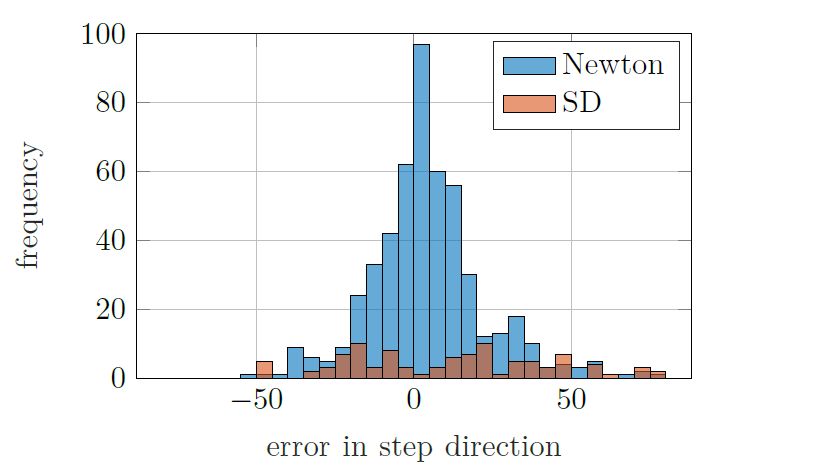
\includegraphics[width=7cm]{figures/newton_SD_direction.png}
		%\caption{Histograms of errors (in angles) between the estimated and true gradient direction and modified Newton step direction when the field measurements are corrupted}
		\label{fig:direction_errors_noise}
	\end{figure}
\begin{itemize}
	\item Corrupt the field strength measurement by +/- 5 percent of the field strength. 
	\item Estimate gradient by collecting local data and solving a least squares problem
	\item Estimate the hessian by collecting data from neighbors and solving another least squares problem
	\item Heuristic: Use Steepest Descent until the estimated hessian is positive definite.
\end{itemize}
\end{frame}
%%%%%%%%%%%%%%%%%%%%%%%%%%%%%%%%%%%%%%%%%%%%%%%%%%%%%%%%%%%%%%%%%%%%%
\subsection{Experimental Results}
%%%%%%%%%%%%%%%%%%%%%%%%%%%%%%%%%%%%%%%%%%%%%%%%%%%%%%%%%%%%%%%%%%%%%
\begin{frame}{Indoor experimental setup}

\begin{minipage}{0.55\textwidth}	
    \begin{figure}[h!]
	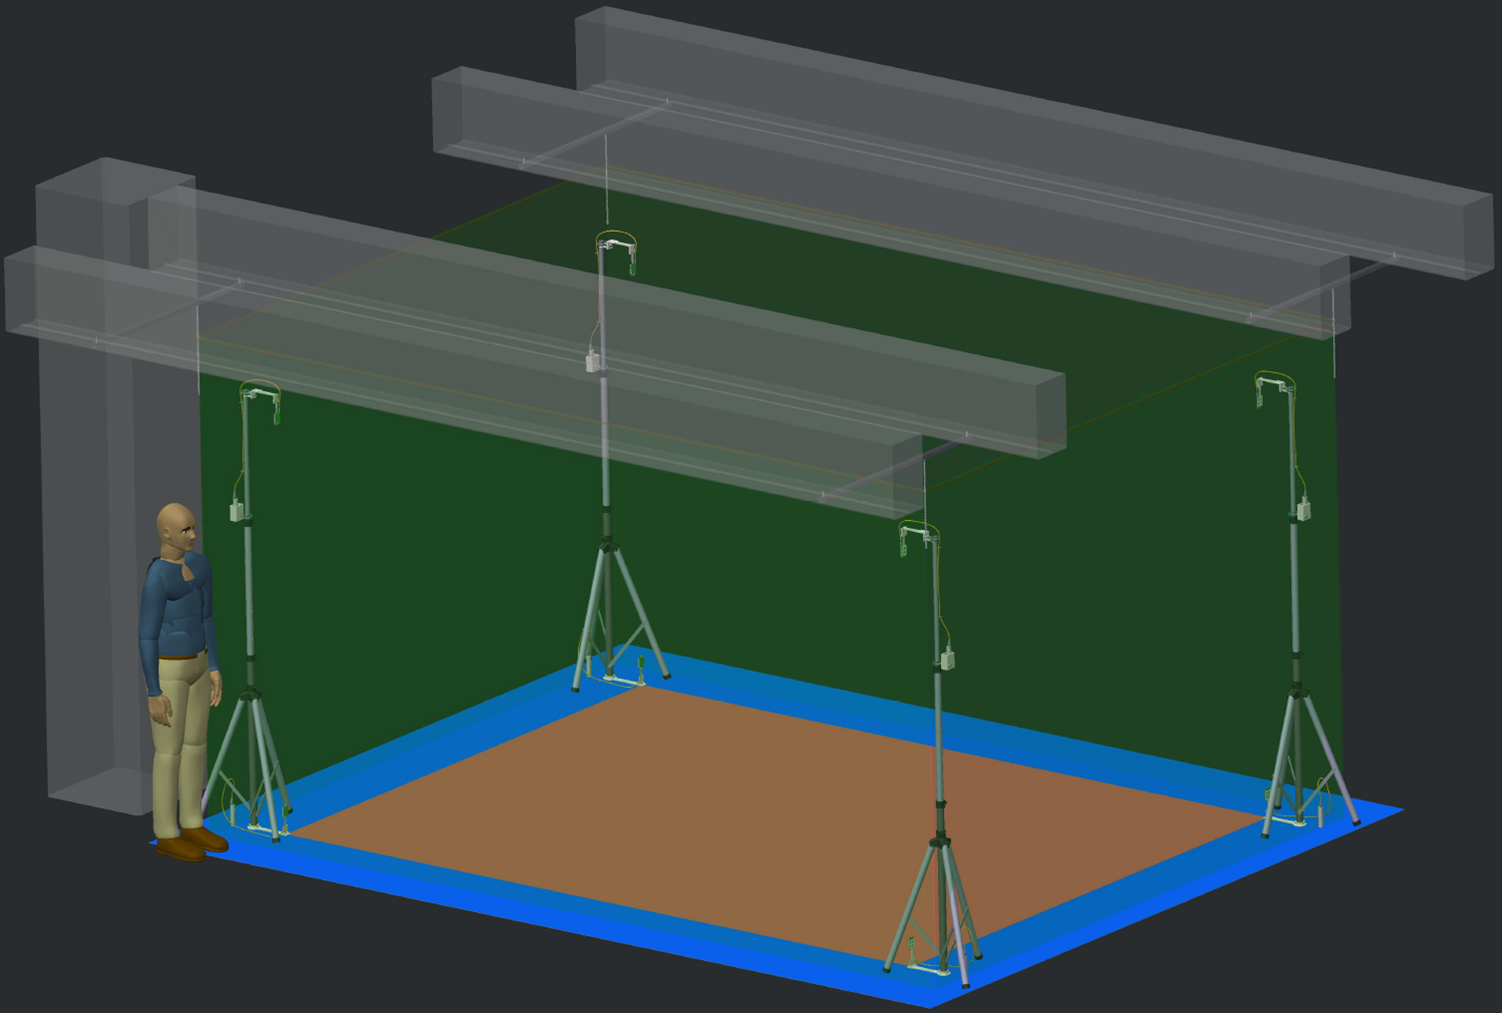
\includegraphics[width=6cm]{figures/LPS_Setup.png}
	\caption{LPS Setup}
	\label{fig:control_arch}	
\end{figure}		
\end{minipage}
	\hspace{0.05cm}
\begin{minipage}{0.35\textwidth}
    \begin{figure}[h!]
	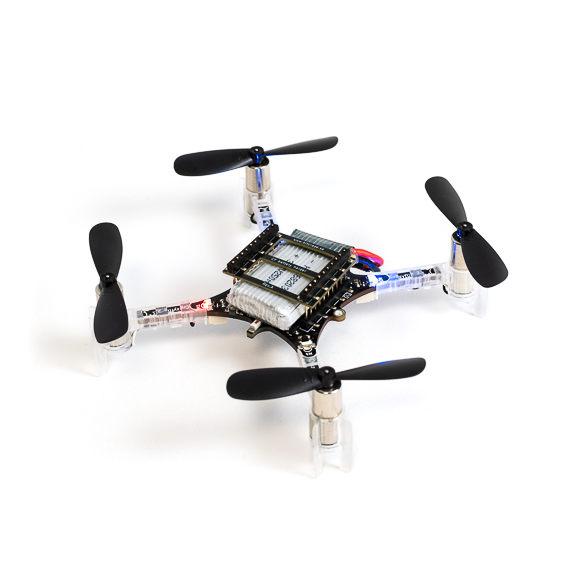
\includegraphics[width=4cm]{figures/crazyflie_2_1_585px.jpg}
	\caption{Crazyflie 2.1}
	\label{fig:control_arch}	
\end{figure}		
\end{minipage}

\begin{itemize}
	\item Indoor Positioning System called the Loco Position System (LPS) and Crazyflie 2.0 developed by the company bitcraze\footnote{https://www.bitcraze.io/products/crazyflie-2-1/}
	\item Implemented a peer-to-peer communication protocol \footnote{Paulsen, 2018.Master thesis.}
\end{itemize}
\end{frame}
%%%%%%%%%%%%%%%%%%%%%%%%%%%%%%%%%%%%%%%%%%%%%%%%%%%%%%%%%%%%%%%%%%%%%%
%\begin{frame}{Experimental results: Quadratic field}
%$\psi(q)=(q-c)^T\begin{bmatrix}1&0\\0&2\end{bmatrix}(q-c)$ with $c=\begin{bmatrix}2\\1.5\end{bmatrix}$
%\vspace{5cm}
%\end{frame}
%%%%%%%%%%%%%%%%%%%%%%%%%%%%%%%%%%%%%%%%%%%%%%%%%%%%%%%%%%%%%%%%%%%%%%
%\begin{frame}{Experimental results: Log-convex field}
%$\psi(q)=-\textnormal{exp}(-||q-c||^2)$ with $c=\begin{bmatrix}2\\1.5\end{bmatrix}$
%\vspace{5cm}	
%\end{frame}
%%%%%%%%%%%%%%%%%%%%%%%%%%%%%%%%%%%%%%%%%%%%%%%%%%%%%%%%%%%%%%%%%%%%%%
%\begin{frame}{Experimental results: Field with two minima}
%$\psi(q)=-\textnormal{exp}(-||q-c_1||^2)-\textnormal{exp}(-||q-c_2||^2)$ with $c_1=\begin{bmatrix}1\\1\end{bmatrix}$, $c_2=\begin{bmatrix}3\\2\end{bmatrix}$
%\vspace{5cm}	
%\end{frame}
%%%%%%%%%%%%%%%%%%%%%%%%%%%%%%%%%%%%%%%%%%%%%%%%%%%%%%%%%%%%%%%%%%%%%%
%\begin{frame}{Visualizing experimental results}
%
%\end{frame}
%%%%%%%%%%%%%%%%%%%%%%%%%%%%%%%%%%%%%%%%%%%%%%%%%%%%%%%%%%%%%%%%%%%%%
% \begin{frame}{Experimental results: Quadratic field}
% 	\textcolor{red}{Replace figure with animation and video} 
% 	\begin{figure}[h!]	
% 		\includegraphics[width=12cm]{figures/quadratic_field_contour.png}
% 		%\caption{Histograms of errors (in angles) between the estimated and true gradient direction and modified Newton step direction when the field measurements are corrupted}
% 		\label{fig:quadratic_field}
% 	\end{figure}
% \end{frame}
%%%%%%%%%%%%%%%%%%%%%%%%%%%%%%%%%%%%%%%%%%%%%%%%%%%%%%%%%%%%%%%%%%%%%
% \begin{frame}{Experimental results: Log-convex field}
% 	\textcolor{red}{Replace figure with animation and video}
% 	\begin{figure}[h!]	
% 		\includegraphics[width=12cm]{figures/log_convex_field_contour.png}
% 		%\caption{Histograms of errors (in angles) between the estimated and true gradient direction and modified Newton step direction when the field measurements are corrupted}
% 		\label{fig:log_convex_field}
% 	\end{figure}
% \end{frame}
%%%%%%%%%%%%%%%%%%%%%%%%%%%%%%%%%%%%%%%%%%%%%%%%%%%%%%%%%%%%%%%%%%%%%
% \begin{frame}{Experimental results: Non-convex field}
% 	\textcolor{red}{Replace figure with animation and video}
% 	\begin{figure}[h!]	
% 		\includegraphics[width=12cm]{figures/non_convex_field_contour.png}
% 		%\caption{Histograms of errors (in angles) between the estimated and true gradient direction and modified Newton step direction when the field measurements are corrupted}
% 		\label{fig:non_convex_field}
% 	\end{figure}
% \end{frame}
%%%%%%%%%%%%%%%%%%%%%%%%%%%%%%%%%%%%%%%%%%%%%%%%%%%%%%%%%%%%%%%%%%%%%%
% \begin{frame}{Experimental Results: Quadratic field(Video)}
% \includemedia[
% activate=pageopen,
% width=300pt,height=200pt,
% addresource=animations/OBLIQUE_quadratic_mod_newton_Fig_4.mp4,
% flashvars={%
% 	src=figures/noObstacle.mp4      % same path as in addresource!
% 	%&scaleMode=stretch % removes black bars
% 	&autoPlay=true      % optional configuration
% 	&loop=true          % variables
% }
% ]{}{StrobeMediaPlayback.swf}
% \end{frame}
% %%%%%%%%%%%%%%%%%%%%%%%%%%%%%%%%%%%%%%%%%%%%%%%%%%%%%%%%%%%%%%%%%%%%%%
% \begin{frame}{Experimental Results: Quadratic field(Animation)}

% 		\includemedia[
% 		activate=pageopen,
% 		width=300pt,height=200pt,
% 		addresource=animations/convex.mp4,
% 		flashvars={%
% 			src=figures/noObstacle.mp4      % same path as in addresource!
% 			%&scaleMode=stretch % removes black bars
% 			&autoPlay=true      % optional configuration
% 			&loop=true          % variables
% 		}
% 		]{}{StrobeMediaPlayback.swf}

% \end{frame}
% %%%%%%%%%%%%%%%%%%%%%%%%%%%%%%%%%%%%%%%%%%%%%%%%%%%%%%%%%%%%%%%%%%%%%%
% \begin{frame}{Experimental Results: Log-Convex quadratic field (Video)}
% 		\includemedia[
% 		activate=pagevisible,
% 		width=300pt,height=200pt,
% 		addresource=animations/OBLIQUEVIEW__log_convex_mod_newton_Fig_5.mp4,
% 		flashvars={%
% 			src=figures/noObstacle.mp4      % same path as in addresource!
% 			%&scaleMode=stretch % removes black bars
% 			&autoPlay=true      % optional configuration
% 			&loop=true          % variables
% 		}
% 		]{}{StrobeMediaPlayback.swf}
% \end{frame}
% %%%%%%%%%%%%%%%%%%%%%%%%%%%%%%%%%%%%%%%%%%%%%%%%%%%%%%%%%%%%%%%%%%%%%%
% \begin{frame}{Experimental Results: Log-Convex quadratic field (Animation)}
% 	\includemedia[
% 	activate=pagevisible,
% 	width=300pt,height=200pt,
% 	addresource=animations/quasiConvex.mp4,
% 	flashvars={%
% 		src=figures/noObstacle.mp4      % same path as in addresource!
% 		%&scaleMode=stretch % removes black bars
% 		&autoPlay=true      % optional configuration
% 		&loop=true          % variables
% 	}
% 	]{}{StrobeMediaPlayback.swf}
% \end{frame}
% %%%%%%%%%%%%%%%%%%%%%%%%%%%%%%%%%%%%%%%%%%%%%%%%%%%%%%%%%%%%%%%%%%%%%%
% \begin{frame}{Experimental Results: Field with multiple minima (Video)}
% 	\includemedia[
% 	activate=pageopen,
% 	width=300pt,height=200pt,
% 	addresource=animations/2 minima mod Newton noise.mp4,
% 	flashvars={%
% 		src=figures/noObstacle.mp4      % same path as in addresource!
% 		%&scaleMode=stretch % removes black bars
% 		&autoPlay=true      % optional configuration
% 		&loop=true          % variables
% 	}
% 	]{}{StrobeMediaPlayback.swf}
% \end{frame}
% %%%%%%%%%%%%%%%%%%%%%%%%%%%%%%%%%%%%%%%%%%%%%%%%%%%%%%%%%%%%%%%%%%%%%%
% \begin{frame}{Experimental Results: Field with multiple minima (Animation)}
% 	\includemedia[
% 	activate=pageopen,
% 	width=300pt,height=200pt,
% 	addresource=animations/2minima.mp4,
% 	flashvars={%
% 		src=figures/noObstacle.mp4      % same path as in addresource!
% 		%&scaleMode=stretch % removes black bars
% 		&autoPlay=true      % optional configuration
% 		&loop=true          % variables
% 	}
% 	]{}{StrobeMediaPlayback.swf}
% \end{frame}
%%%%%%%%%%%%%%%%%%%%%%%%%%%%%%%%%%%%%%%%%%%%%%%%%%%%%%%%%%%%%%%%%%%%%
%%\subsection{Conclusion}
%%%%%%%%%%%%%%%%%%%%%%%%%%%%%%%%%%%%%%%%%%%%%%%%%%%%%%%%%%%%%%%%%%%%%
\begin{frame}{Conclusions and ongoing work}
Conclusions:
\begin{itemize}
    \item Proposed a distributed control algorithm to address the source-seeking probem
    \item Analyzed the convergence properties
    \item Presented experimental results
\end{itemize}
Ongoing Work:
\begin{itemize}
    \item Consider general non-linear agent dynamics instead of approximating it as a single integrator\footnote{A.  Attallah,  A.  Datar,  and  H.  Werner,  “Flocking  of  linear  parametervarying agents: Source seeking application with underwater vehicles (To be presented at IFAC 2020).}
    \item Consider level-tracking scenarios
    % \footnote{\textcolor{red}{Preliminary results: youtube link}}
\end{itemize}
\end{frame}
%%%%%%%%%%%%%%%%%%%%%%%%%%%%%%%%%%%%%%%%%%%%%%%%%%%%%%%%%%%%%%%%%%%%%
\subsection{(Speculative) Extension to non-linear/uncertain agents} 
%%%%%%%%%%%%%%%%%%%%%%%%%%%%%%%%%%%%%%%%%%%%%%%%%%%%%%%%%%%%%%%%%%%%%
%%%%%%%%%%%%%%%%%%%%%%%%%%%%%%%%%%%%%%%%%%%%%%%%%%%%%%%%%%%%%%%%%%%%%
\subsubsection{Double integrator agents to general non-linear agents}
\begin{frame}{Double integrator agents to general non-linear agents}
	\begin{figure}[h!]
		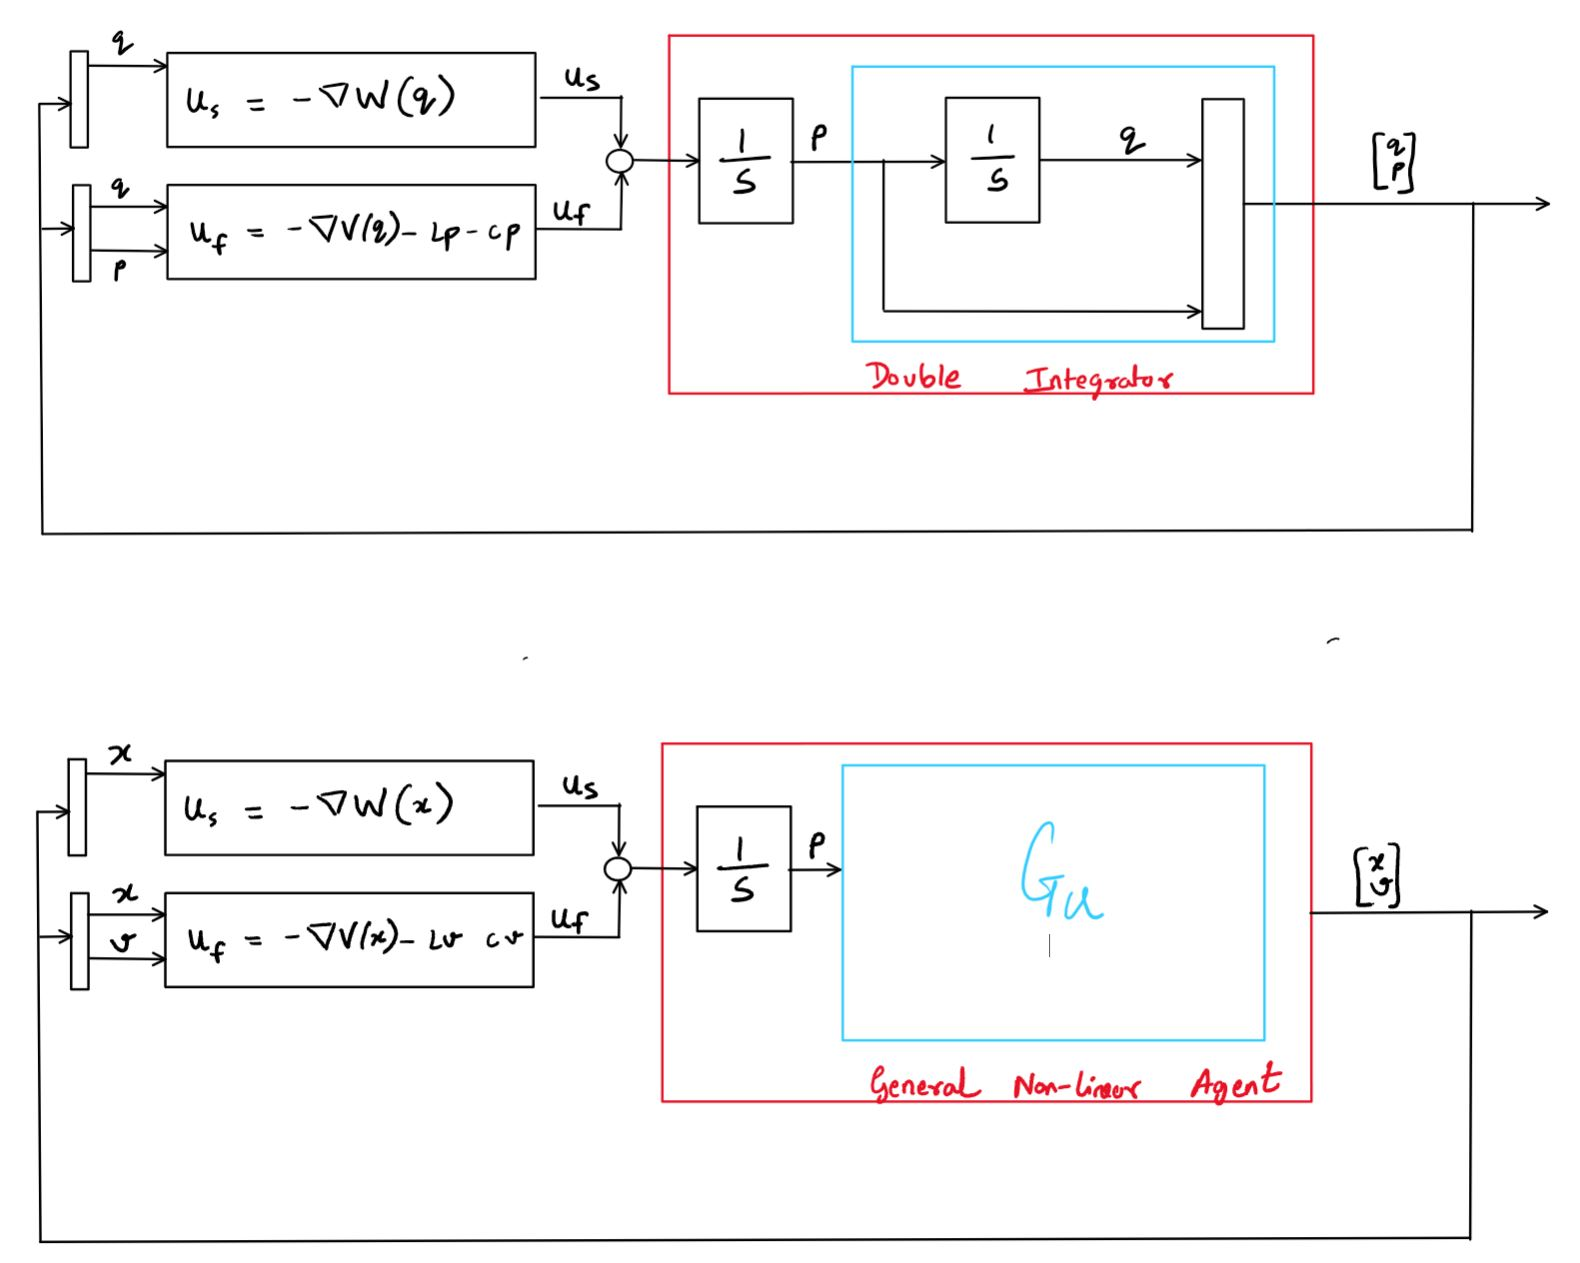
\includegraphics[width=10cm]{doc/1_Flocking_source_seek/double_integrator_to_general_agents_slide.jpg}
		%\caption{}
		\label{fig:control_arch}	
	\end{figure}	
\end{frame}
%%%%%%%%%%%%%%%%%%%%%%%%%%%%%%%%%%%%%%%%%%%%%%%%%%%%%%%%%%%%%%%%%%%%%
\begin{frame}{Double integrator agents to general non-linear agents}
Dynamics with double integrator:
\begin{equation*}
\begin{split}
\Dot{q}&=p\\
\Dot{p}&=-\nabla V(q)-\hat{L}(q)p -cp\textcolor{red}{-k_1\nabla^2 \Psi(q) p -k_2 \nabla \Psi(q)}
\end{split}
\end{equation*}	
Dynamics with general agents:
\begin{equation*}
\begin{split}
\begin{bmatrix}
x\\v
\end{bmatrix}&=G_{\textnormal{cl}}p\\
\Dot{q}&=p\\
\Dot{p}&=-\nabla V(\textcolor{blue}{x})-\hat{L}(\textcolor{blue}{x})\textcolor{blue}{v} -c\textcolor{blue}{v}\textcolor{red}{-k_1\nabla^2 \Psi(\textcolor{blue}{x}) \textcolor{blue}{v} -k_2 \nabla \Psi(\textcolor{blue}{x})}
\end{split}
\end{equation*}			
\end{frame}
%%%%%%%%%%%%%%%%%%%%%%%%%%%%%%%%%%%%%%%%%%%%%%%%%%%%%%%%%%%%%%%%%%%%%
\begin{frame}{Double integrator agents to general non-linear agents}
\textbf{Core Idea:}
\\
Under  
\begin{itemize}
\item a Lipschitz condition on the underlying scalar field 
\item a Lipschitz condition on the interaction field
\item $L_2$ bound on the tracking error of the local closed loop, $G_{\textnormal{cl}}$
\end{itemize}
the dynamics for general agents could be written as:
\begin{equation*}
\begin{split}
\Dot{q}&=p\\
\Dot{p}&=-\nabla V(q)-\hat{L}(q)p -cp\textcolor{red}{-k_1\nabla^2 \Psi(q) p -k_2 \nabla \Psi(q)} + \textcolor{blue}{d}\\
||d_T||&\leq K ||p_T||_{L_2} \forall T
\end{split}
\end{equation*}	
\begin{itemize}
\item Standard dissipativity based arguments to show stability (Boundedness of trajectories)
\item Assymptotic stability not shown !
\end{itemize}
\end{frame}
%%%%%%%%%%%%%%%%%%%%%%%%%%%%%%%%%%%%%%%%%%%%%%%%%%%%%%%%%%%%%%%%%%%%%
\begin{frame}{Double integrator agents to general non-linear agents}
A speculative idea
\begin{itemize}
	\item IQCs can be used efficiently to get upper bounds on robust exponential decay rates\footnote{Boczar, R., Lessard, L., Packard, A. and Recht, B., 2017. Exponential stability analysis via integral quadratic constraints. arXiv preprint arXiv:1706.01337.}
	\item Can be possibly applied to LPV systems to obtain exponential decay rates under parameter variation
	\item These rates could be then used with a singular perturbation and a regular perturbation argument to prove asymptotic stability of the overall system
	\item The linear analogue would be to consider the slowest eigen values of the closed loop agent dynamics
\end{itemize}
\end{frame}
%%%%%%%%%%%%%%%%%%%%%%%%%%%%%%%%%%%%%%%%%%%%%%%%%%%%%%%%%%%%%%%%%%%%%
\begin{frame}{Other speculative ideas}
	\
	\begin{itemize}
		\item Adapt the flocking algorithm coefficients online based on the measured error such the $\dot{E}<0$. (Borrowing ideas from adaptive control)
		\item Similar to ideas in \footnote{Chopra, N. and Spong, M.W., 2006. Passivity-based control of multi-agent systems. In Advances in robot control (pp. 107-134). Springer, Berlin, Heidelberg.}, design local tracking control for passivity and use the fact the interconnections of passive systems is passive.
	\end{itemize}
\end{frame}
%%%%%%%%%%%%%%%%%%%%%%%%%%%%%%%%%%%%%%%%%%%%%%%%%%%%%%%%%%%%%%%%%%%%%
%\section{Formation Stabilization with a decoupled architecture}
%\subsection{Problem}
%%%%%%%%%%%%%%%%%%%%%%%%%%%%%%%%%%%%%%%%%%%%%%%%%%%%%%%%%%%%%%%%%%%%%
\begin{frame}{Formation forming problem}
\begin{figure}
	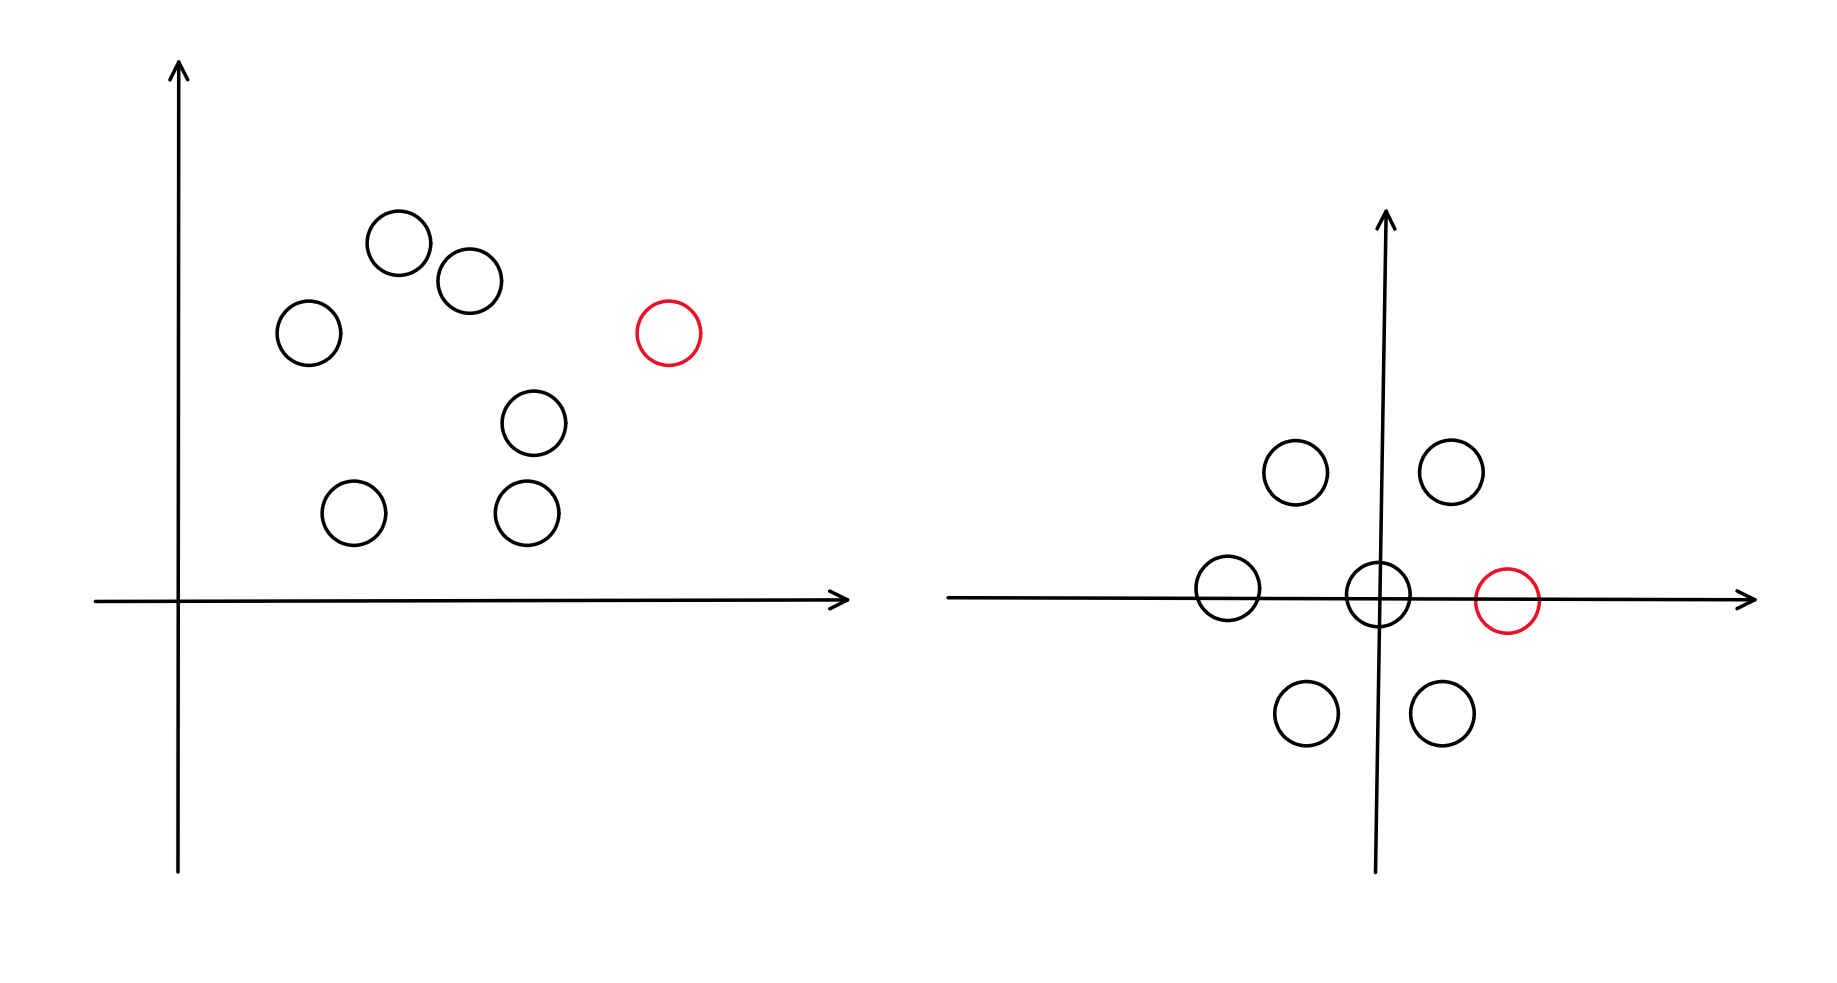
\includegraphics[width=0.55\textwidth]{figures/formation_control_schematic.png}
	%\caption{Oil Spills}
	%\label{fig:oilspills}
\end{figure}
\begin{itemize}
	\item A group of $N$ agents randomly deployed
	\item A single agent is externally "informed" (or controlled) to a desired location over time
	\item Each agent knows its $ID$ its desired offset from a commonly agreed location
	\item The dynamics of the complete system can be divided into
	\begin{itemize}
		\item Information flow dynamics over the network
		\item Local physical agent dynamics
	\end{itemize}	
\end{itemize}
\end{frame}
%%%%%%%%%%%%%%%%%%%%%%%%%%%%%%%%%%%%%%%%%%%%%%%%%%%%%%%%%%%%%%%%%%%%%
\begin{frame}{Core idea and key question}
	\begin{itemize}
		\item Vast literature on first order protocols (information flow dynamics)
		\item Real agents typically have higher order models
		\item \textbf{Core idea:} Wrap local tracking controller around simple information flow dynamics \footnote{Cortés, J. and Egerstedt, M., 2017. Coordinated control of multi-robot systems: A survey. SICE Journal of Control, Measurement, and System Integration, 10(6), pp.495-503.}
		\item \textbf{Core question:} Can we derive theoretical bounds on the loss in performance that depend on the local tracking performance?
	\end{itemize}
\end{frame}
%%%%%%%%%%%%%%%%%%%%%%%%%%%%%%%%%%%%%%%%%%%%%%%%%%%%%%%%%%%%%%%%%%%%%
\begin{frame}{Decoupled control Architecture}
	\begin{figure}[h!]
		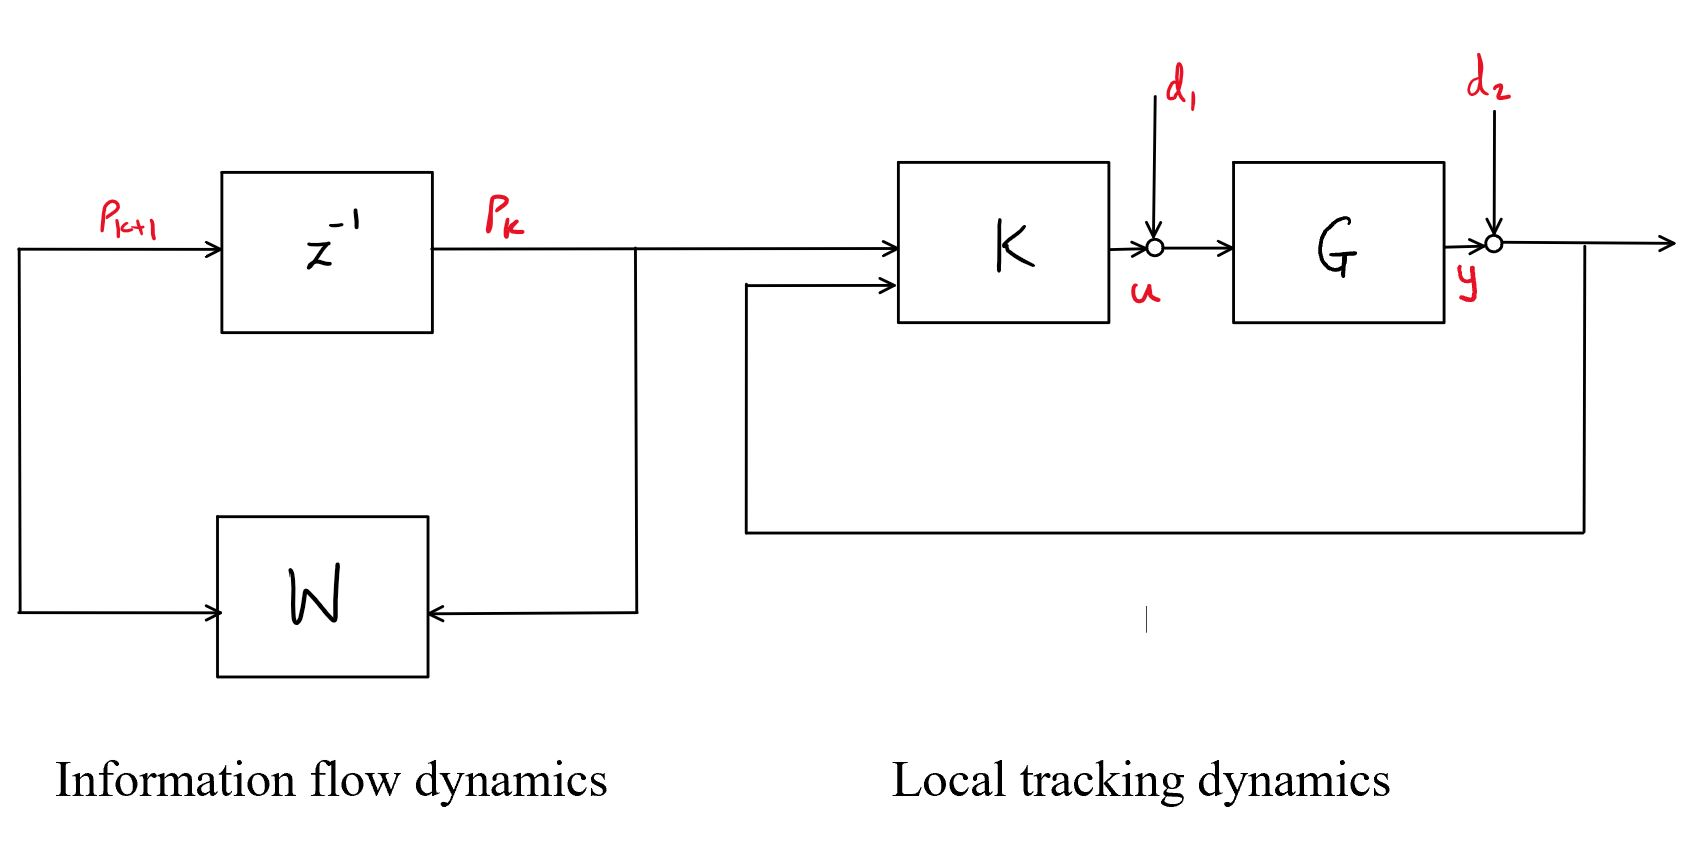
\includegraphics[width=10cm]{doc/2_Formation_control/decoupled_architecture.jpg}
		%\caption{}
		\label{fig:control_arch}	
	\end{figure}
Information flow dynamics
	\begin{equation*}\label{eqn:perturbed_information_flow_dynamics}
	\begin{split}
	p_{k+1}=W_cp_k \\
	\end{split}
	\end{equation*}
Physical agent dynamics (closed loop)	
	\begin{equation*}
	\begin{split}	
	\forall i \in \{1,\cdots, N\}:
	~~&\left\{
	\begin{array}{ll}
	x_i(k+1)&=Ax_i(k)+B_pp_i(k) + \bar{B}_dd_i(k) \\
	y_i(k) &=C1x_i(k) 
	\end{array}
	\right.
	\end{split}
	\end{equation*}
\end{frame}
%%%%%%%%%%%%%%%%%%%%%%%%%%%%%%%%%%%%%%%%%%%%%%%%%%%%%%%%%%%%%%%%%%%%%
\begin{frame}{Theory}
\begin{itemize}
	\item Scalable Analysis of information flow dynamics -> Positive systems theory\footnote{Rantzer, A., 2011, December. Distributed control of positive systems. In 2011 50th IEEE Conference on Decision and Control and European Control Conference (pp. 6608-6611). IEEE.}
	\item Local tracking loop Analysis -> generalized $H_2$ norm (induced $l_2$ to $l_{\infty}$ norm for non-linear systems)
	\item Scalable Analysis and Synthesis result
\end{itemize}
\end{frame}
%%%%%%%%%%%%%%%%%%%%%%%%%%%%%%%%%%%%%%%%%%%%%%%%%%%%%%%%%%%%%%%%%%%%%
\begin{frame}{Some simulation results}
	\begin{minipage}{0.45\textwidth}	
		\begin{figure}
			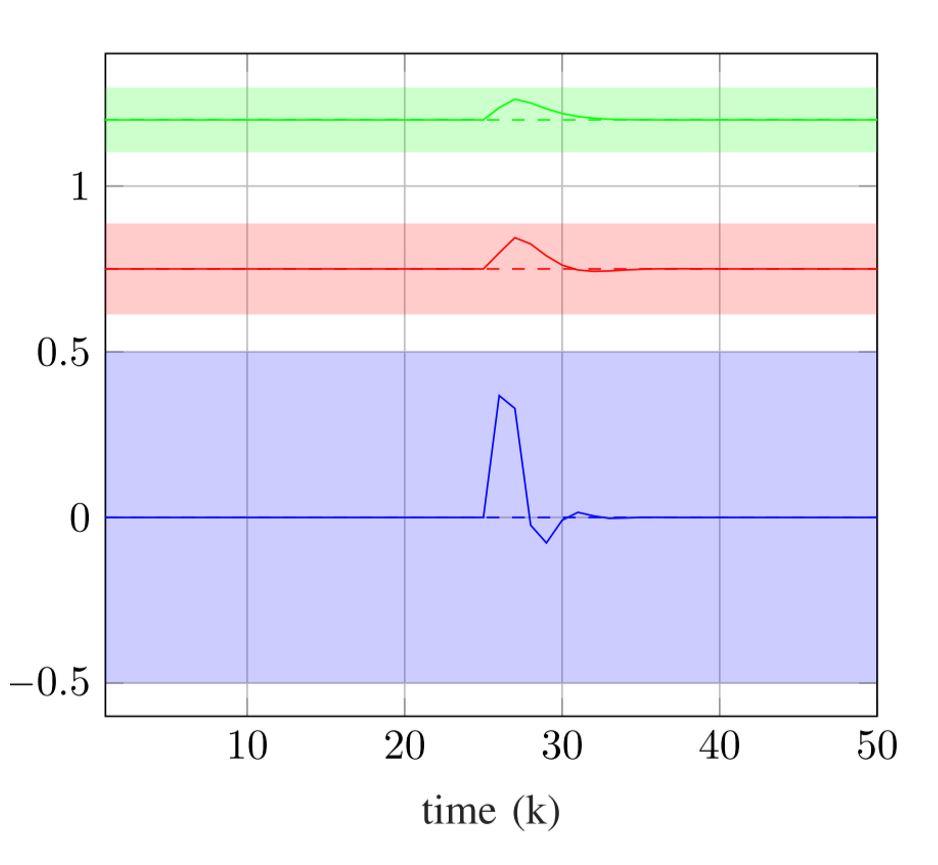
\includegraphics[width=1\textwidth]{doc/2_Formation_control/dist_rejection.jpg}
			%\caption{Fukushima Disaster (2011)}
			%\label{fig:fukushima_disaster}
		\end{figure}
		\begin{itemize}
			\item Disturbance rejection 
			\item Guaranteed peak bounds
		\end{itemize}		
	\end{minipage}
	\begin{minipage}{0.45\textwidth}	
		\begin{figure}
			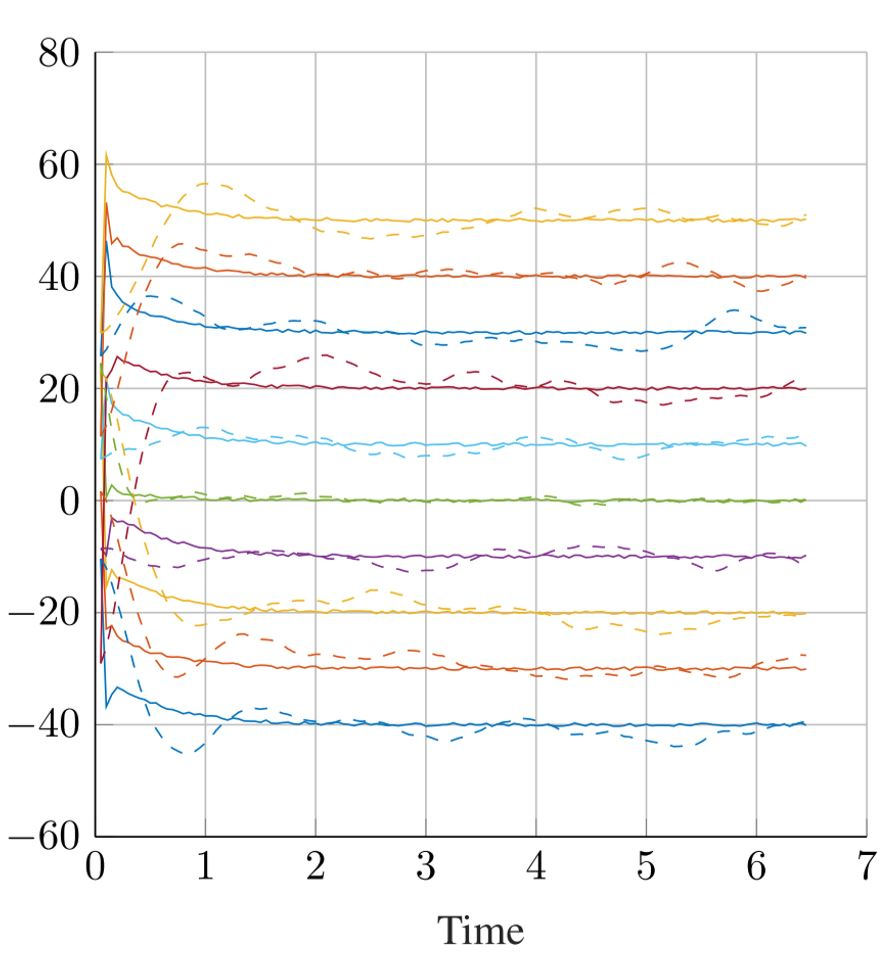
\includegraphics[width=1\textwidth]{doc/2_Formation_control/formation_stabilization.jpg}
			%\caption{Fukushima Disaster (2011)}
			%\label{fig:fukushima_disaster}
		\end{figure}
		\begin{itemize}
			\item Formation stabilization
		\end{itemize}		
	\end{minipage}	
\end{frame}	
%%%%%%%%%%%%%%%%%%%%%%%%%%%%%%%%%%%%%%%%%%%%%%%%%%%%%%%%%%%%%%%%%%%%%
\begin{frame}{Extensions to lossy networks}
	\begin{figure}[h!]
		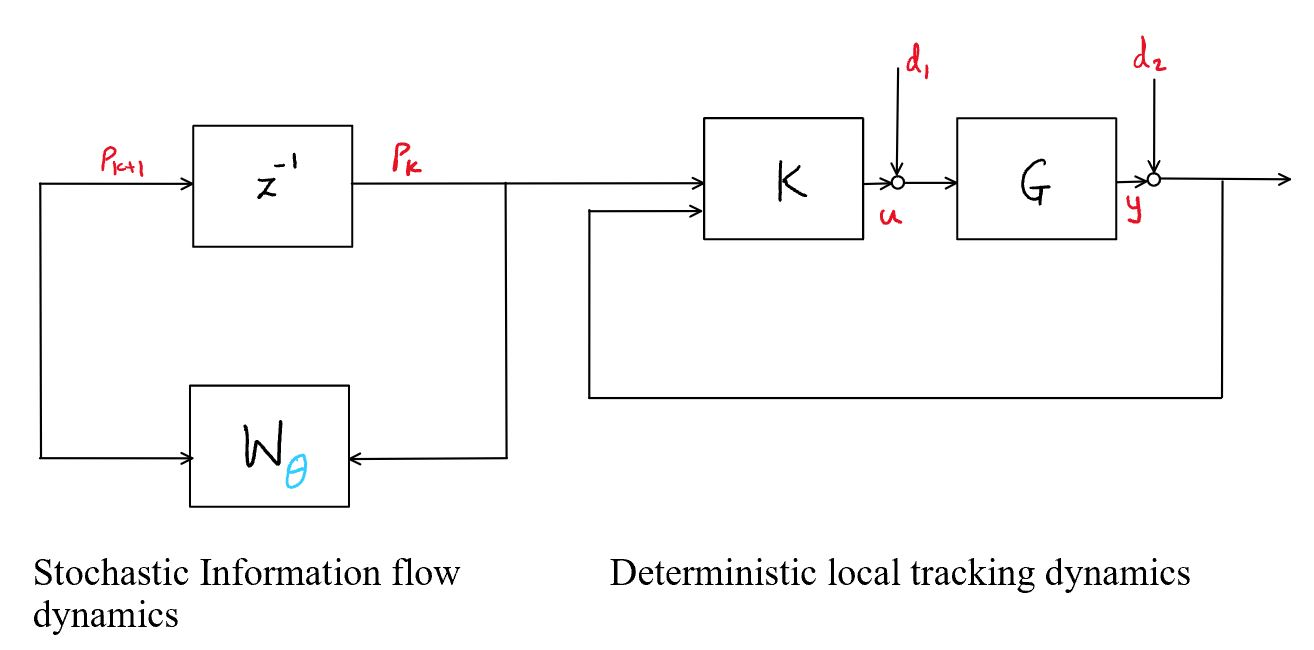
\includegraphics[width=9cm]{doc/2_Formation_control/stoch_decoupled_architecture.jpg}
		%\caption{}
		\label{fig:control_arch}	
	\end{figure}
	Stochastic information flow dynamics
	\begin{equation*}\label{eqn:perturbed_information_flow_dynamics}
	\begin{split}
	p_{k+1}=W_{\theta_k}p_k \\
	\end{split}
	\end{equation*}
	where $\{\theta_k\}_k$ is a finite Markov process 
	\begin{itemize}
		\item Want to derive LMIs to guarante performance e.g mean-square stability of the overall system
	\end{itemize}
\end{frame}
%%%%%%%%%%%%%%%%%%%%%%%%%%%%%%%%%%%%%%%%%%%%%%%%%%%%%%%%%%%%%%%%%%%%%

%\subsection{Theory}
%%%%%%%%%%%%%%%%%%%%%%%%%%%%%%%%%%%%%%%%%%%%%%%%%%%%%%%%%%%%%%%%%%%%%
\begin{frame}{Information flow dynamics: Structure of $\bar{W}_c$}
\begin{figure}
	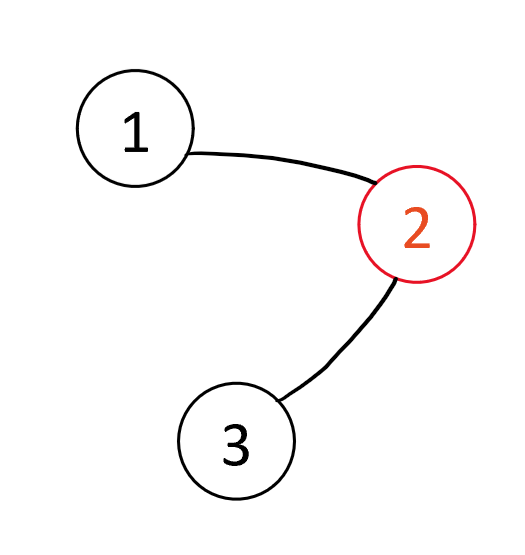
\includegraphics[width=0.3\textwidth]{figures/info_dyn_example.png}
	%\caption{Oil Spills}
	%\label{fig:oilspills}
\end{figure}
\begin{equation*}
\begin{split}
p_{k+1}&=\bar{W}_cp_k\\
&=\begin{bmatrix}
w_{11} & w_{12}&0\\
w_{21} & w_{22}&w_{22}\\
0 & w_{32}&w_{33}\\
\end{bmatrix}p_k
\end{split}
\end{equation*}
\begin{itemize}
\item Lot of work on designing weights for consensus e.g Metropolis-Hastings, equal-neighbor etc
\item We assume $w_{ij}\geq 0$ (Might be restrictive)
\end{itemize}
\end{frame}
%%%%%%%%%%%%%%%%%%%%%%%%%%%%%%%%%%%%%%%%%%%%%%%%%%%%%%%%%%%%%%%%%%%%%
\begin{frame}{Analysis of large scale positive systems}
	\textbf{\footnote{Rantzer, 2018}Theorem 1:}
	Consider a discrete-time autonomous system governed by 
	\begin{equation*}
	\begin{split}
	p_{k+1}=\bar{W}_cp_k, \\
	\end{split}
	\end{equation*}
	where $\bar{W}_c\geq 0$.		
	
	The following statements are equivalent
	\begin{itemize}
		\setlength\itemsep{0.3em}
		\item[(1)] $\bar{W}_c$ is Schur
		\item[(2)] $\lim\limits_{k\rightarrow \infty} p_k=\mathbf{0} \hspace{0.2cm} \forall p_0 \in \mathbb{R}^{n_p}$
		\item[(3)] $\exists \textnormal{ diagonal }P \succ 0 :\ P- \bar{W}_c^TP\bar{W}_c \succ 0$
		\item[(4)] $\exists \textnormal{ diagonal } P:\ \begin{bmatrix}
		P & \bar{W}_c^TP \\
		P\bar{W}_c& P
		\end{bmatrix} \succ 0$
	\end{itemize}	
\end{frame}
%%%%%%%%%%%%%%%%%%%%%%%%%%%%%%%%%%%%%%%%%%%%%%%%%%%%%%%%%%%%%%%%%%%%%
\begin{frame}{Scalable analysis}
\begin{itemize}	
	\item Diagonal P preserves the sparsity pattern in $\begin{bmatrix}
	P & \bar{W}_c^TP \\
	P\bar{W}_c& P
	\end{bmatrix}$
	\item Decompose the feasibility problem into small problems 
	\\(Uses the theory of chordal graphs and chordal graph extensions)\footnote{Papachristodoulou et al., 2012}
\end{itemize}
\end{frame}
%%%%%%%%%%%%%%%%%%%%%%%%%%%%%%%%%%%%%%%%%%%%%%%%%%%%%%%%%%%%%%%%%%%%%
\begin{frame}{Local analysis of agent dynamics}
\textcolor{blue}{Dynamics of agent $i$:}
\begin{equation*}
\begin{split}	
\begin{array}{ll}
x^i_{k+1}&=\bar{A}x^i_k+\bar{B}_pp^i_{k+1} + \bar{B}_ww^i_k \\
y^i_k &=\bar{C}x^i_k 
\end{array}
\end{split}
\end{equation*}
\pause
\textcolor{blue}{Generalized plant for agent $i$:}
\begin{figure}
	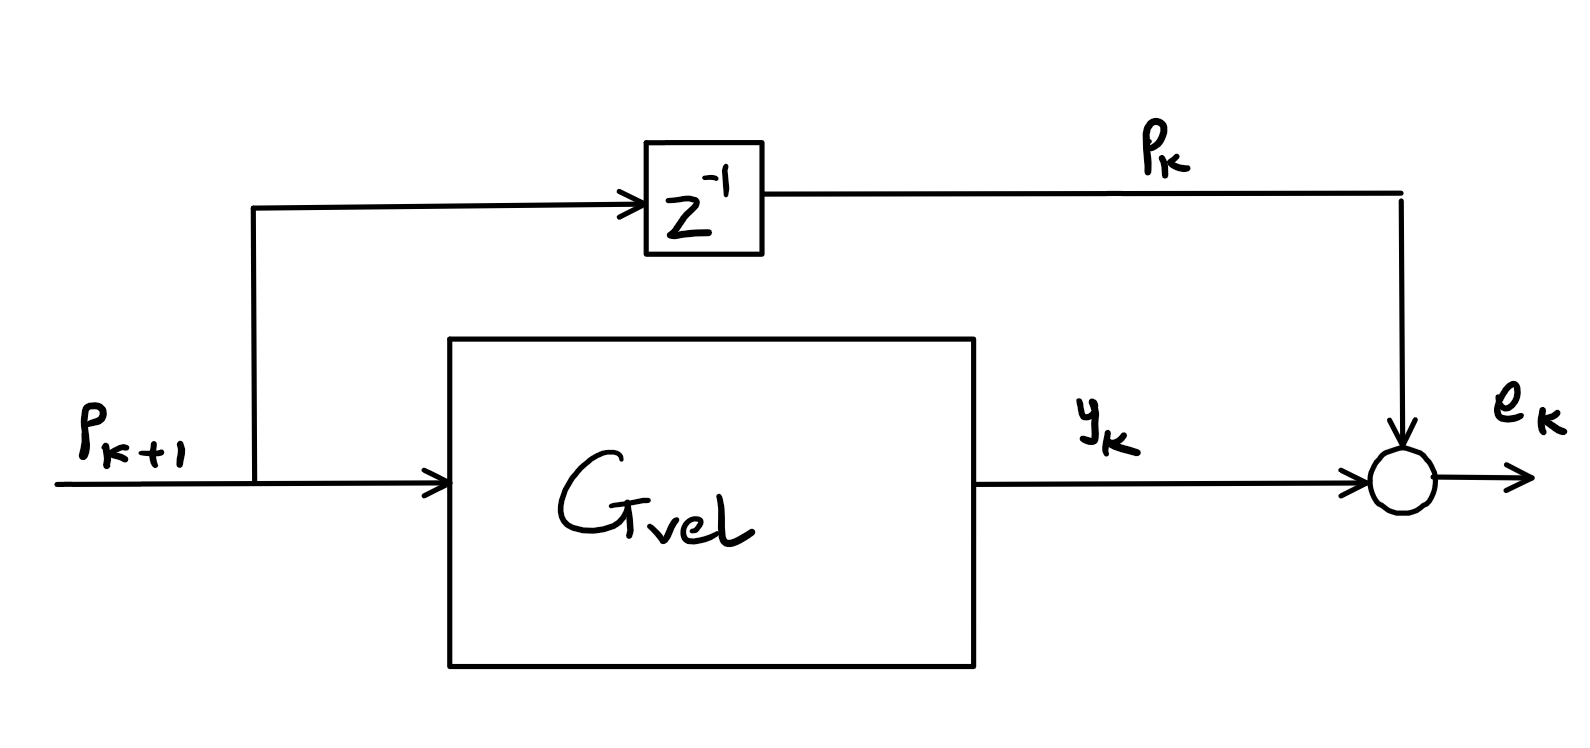
\includegraphics[width=0.45\textwidth]{figures/gen_plant_tf.png}
	%\caption{Oil Spills}
	%\label{fig:oilspills}
\end{figure}
\begin{equation*}\label{complete_closed_loop_aug_system}
\begin{split}
\begin{bmatrix}
z^i_{k+1}\\
\bar{z}^i_{k+1}
\end{bmatrix}
&=
\begin{bmatrix}
\bar{A} & 0\\
0 & 0\\
\end{bmatrix}
\begin{bmatrix}
z^i_k\\
\bar{z}^i_k
\end{bmatrix}
+
\begin{bmatrix}
\bar{B}_p\\
I 
\end{bmatrix}
p^i_{k+1}
+
\begin{bmatrix}
\bar{B}_w\\
0
\end{bmatrix}
w^i_k\\
\\
e^i_k &=
\begin{bmatrix}
-\bar{C} & I
\end{bmatrix}
\begin{bmatrix}
z^i_k\\
\bar{z}^i_k
\end{bmatrix}
\end{split}
\end{equation*}
\end{frame}
%%%%%%%%%%%%%%%%%%%%%%%%%%%%%%%%%%%%%%%%%%%%%%%%%%%%%%%%%%%%%%%%%%%%%
\begin{frame}{Local $l_2$ to $l_{\infty}$ control}
\textcolor{blue}{Generalized plant:}
\begin{equation}\label{eqn_open_loop_system}
\begin{split}
\eta_{k+1}&=\mathcal{A}\eta_k+\mathcal{B}_pp_k+\mathcal{B}_ww_k, \hspace{0.2cm}\eta_0=0\\
e_k &=\mathcal{C}\eta_k 
\end{split}
\end{equation}	
\pause
\textbf{Theorem 2:}
	For a discrete-time dynamical system governed by \eqref{eqn_open_loop_system}, 
	if $\exists K\succ0$, $\gamma_p \geq0$, $\gamma_w\geq0$ such that 
	\begin{equation} \label{eqn_LMI_Dissipativity1}
	\begin{split}	
	\hspace{1cm}
	\begin{bmatrix}
	\mathcal{A}^T\\
	\mathcal{B}_p^T\\
	\mathcal{B}_w^T\\
	\end{bmatrix}
	K
	\begin{bmatrix}
	\mathcal{A} & \mathcal{B}_p & \mathcal{B}_w
	\end{bmatrix}
	&\prec
	\begin{bmatrix}
	K & 0 & 0\\
	0 & \gamma_p^2 I&0\\
	0 & 0 &\gamma_w^2 I\\
	\end{bmatrix}\\
	\end{split}
	\end{equation}
	and
	\begin{equation}\label{eqn_LMI_output_bound1}
	\begin{bmatrix}
	K & \mathcal{C}^T \\
	* & I \\
	\end{bmatrix}\succ0, 
	\end{equation}
	then
	\begin{equation*}
	||e_k||_2^2\leq  \gamma_p^2||p||_{l_2}^2+\gamma_w^2||w||_{l_2}^2  \hspace{0.4cm} \forall w,p \in l_2,\ \forall k.
	\end{equation*}
\end{frame}
%%%%%%%%%%%%%%%%%%%%%%%%%%%%%%%%%%%%%%%%%%%%%%%%%%%%%%%%%%%%%%%%%%%%%
\begin{frame}{Local $l_2$ to $l_{\infty}$ control for agents}
\textbf{Proof:}	
	Condition (\ref{eqn_LMI_Dissipativity1}) is equivalent to the existence of $\epsilon>0$ such that $\forall \eta_k \in \mathbb{R}^{n_\eta},\forall w_k \in \mathbb{R}^{n_w}$, $\forall p_k \in \mathbb{R}^{n_p}$,
	\begin{equation*}
	\eta_{k+1}^TK\eta_{k+1}\leq\eta_{k}^TK\eta_{k}+(\gamma_p^2-\epsilon) ||p_{k}||_2^2+(\gamma_w^2-\epsilon) ||w_{k}||_2^2.
	\end{equation*}
	\pause
	Defining the storage function  $V_k=\eta_k^TK\eta_k$, we have  $\forall w_k \in \mathbb{R}^{n_w}$ and $\forall p_k \in \mathbb{R}^{n_p}$, 
	\begin{equation*}
	\begin{split}
	V_{k+1}&\leq V_{k}+\gamma_p^2 ||p_{k}||_2^2+\gamma_w^2 ||w_{k}||_2^2\\
	\pause
	&\leq V_{0}+\gamma_p^2 \sum_{i=0}^{k}||p_{i}||_2^2+\gamma_w^2 \sum_{i=0}^{k}||w_{i}||_2^2
	\end{split}	
	\end{equation*}
	\pause
	With zero initial conditions, and $\forall w,p \in l_2$, 
	\begin{equation} \label{eqn_dissipativity}
	V_{k}\leq\gamma_p^2\sum_{i=0}^{k-1}||p_i||_2^2+\gamma_w^2\sum_{i=0}^{k-1}||w_i||_2^2\leq\gamma_p^2||p||_{l_2}^2+\gamma_w^2||w||_{l_2}^2. 
	\end{equation}
\end{frame}
%%%%%%%%%%%%%%%%%%%%%%%%%%%%%%%%%%%%%%%%%%%%%%%%%%%%%%%%%%%%%%%%%%%%%
\begin{frame}{Local $l_2$ to $l_{\infty}$ control for agents}
\textbf{Proof(ctd):} Condition (\ref{eqn_LMI_output_bound1}) can be converted using the Schur complement to
\begin{equation}
K-C^TC\succ0
\end{equation}
which is equivalent to 
\begin{equation*}
V_k=\eta_k^TK\eta_k\geq\eta_k^TC^TC\eta_k=e_k^Te_k \hspace{0.3cm}\forall \eta_k \in \mathbb{R}^{n_\eta}
\end{equation*}
which together with equation (\ref{eqn_dissipativity}) implies 
\begin{equation*}
||e_k||_2^2\leq V_k \leq \gamma_p^2||p||_{l_2}^2+\gamma_w^2||w||_{l_2}^2.  
\end{equation*}
$\forall w,p \in l_2$, $\forall k$
\end{frame}
%%%%%%%%%%%%%%%%%%%%%%%%%%%%%%%%%%%%%%%%%%%%%%%%%%%%%%%%%%%%%%%%%%%%%
\begin{frame}{Complete interconnected system: Analysis}
\begin{equation}\label{eqn:full_system_closed_loop}
\begin{split}
&\hspace{0.78cm}p_{k+1}=\bar{W}_cp_k \\
\forall i:
~~&\left\{
\begin{array}{ll}
x^i_{k+1}&=\bar{A}x^i_k+\bar{B}_pp^i_{k+1} + \bar{B}_ww^i_k \\
y^i_k &=\bar{C}x^i_k 
\end{array}
\right.
\end{split}
\end{equation}
For the interconnected system (\ref{eqn:full_system_closed_loop}), consider the following three LMIs:
\begin{equation} \label{eqn_LMI_pos_analysis}
%\exists \textnormal{ diagonal } P :
\left[
\begin{array}{c|c}
\alpha^2 P & \bar{W}_c^TP \\
\hline \\
P\bar{W}_c& P
\end{array}\right] \succ 0,
\end{equation} 
\begin{equation} \label{eqn_LMI_Dissipativity}
\begin{split}	
\hspace{1cm}
\begin{bmatrix}
\mathcal{A}^T\\
\mathcal{B}_p^T\\
\mathcal{B}_w^T\\
\end{bmatrix}
K
\begin{bmatrix}
\mathcal{A} & \mathcal{B}_p & \mathcal{B}_w
\end{bmatrix}
&\prec
\begin{bmatrix}
K & 0 & 0\\
0 & \gamma_p^2 I&0\\
0 & 0 &\gamma_w^2 I\\
\end{bmatrix}\\
\end{split}
\end{equation}
\begin{equation}\label{eqn_LMI_output_bound}
\begin{bmatrix}
K & \mathcal{C}^T \\
* & I \\
\end{bmatrix}\succ0, 
\end{equation}
\end{frame}
%%%%%%%%%%%%%%%%%%%%%%%%%%%%%%%%%%%%%%%%%%%%%%%%%%%%%%%%%%%%%%%%%%%%%
\begin{frame}{Complete interconnected system: Analysis}
\textbf{Theorem 3:} If for $0\leq \alpha< 1$, $\exists P$ diagonal and $\exists K \succ 0$ and $\gamma_p\geq0$, $\gamma_w\geq0$ such that the LMIs \eqref{eqn_LMI_pos_analysis}, \eqref{eqn_LMI_Dissipativity} and \eqref{eqn_LMI_output_bound} are satisfied,
then the interconnected system is stable such that for all bounded disturbances $||w^i||_{l_2}\leq \beta$,
\begin{equation}\label{eqn:stability guarantee}
||y_k^i||_2\leq (\alpha^k+\frac{\gamma_p}{1-\alpha})\sqrt{\textnormal{cond}(P)}||p_0||_2+\gamma_w\beta
\end{equation} $\forall k$.

Moreover
\begin{equation}\label{perf_bound1}
\begin{split}
\nu_k\leq\mu_k+\frac{\gamma_p}{1-\alpha}\sqrt{\frac{\textnormal{cond}(P)}{N}}||p_0||_2+\gamma_w\beta.
\end{split}
\end{equation}	
and 
\begin{equation}\label{perf_bound2}
J_k\leq M_k+\alpha^{2k}\frac{d_{\textnormal{max}}\gamma_p^2}{|\mathcal{E}|}\textnormal{cond}(P)||p_0||_2^2+\gamma_w^2 \beta^2.
\end{equation}
\end{frame}
%%%%%%%%%%%%%%%%%%%%%%%%%%%%%%%%%%%%%%%%%%%%%%%%%%%%%%%%%%%%%%%%%%%%%
\begin{frame}{Complete interconnected system: Analysis}
\textbf{Key arguments in the proof}
\begin{itemize}
\item Application of Theorem 1 and Theorem 2
\item Convergence result of geometric series
\item Other estimates on norms such as $\frac{1}{\sqrt{N}}||p||_1\leq||p_k||_2\leq||p_k||_1$
\end{itemize}
\end{frame}
%%%%%%%%%%%%%%%%%%%%%%%%%%%%%%%%%%%%%%%%%%%%%%%%%%%%%%%%%%%%%%%%%%%%%
\begin{frame}{Analysis to Synthesis}

Conisder the control variable matrices $F_1$, $F_2$ and a diagonal matrix $E$ of appropriate sizes forming the closed loop matrices
\begin{itemize}
\item $\bar{W}_c=I-EL_c$ where $L_c$ is the perturbed Laplacian matrix
\item $\bar{A}=A+B_uF_1$
\item $\bar{B}_p=B_uF_2$
\end{itemize}	
\end{frame}
%%%%%%%%%%%%%%%%%%%%%%%%%%%%%%%%%%%%%%%%%%%%%%%%%%%%%%%%%%%%%%%%%%%%%
\begin{frame}{Analysis to Synthesis}
	Now consider the set of LMIs:
	\begin{equation}\label{eqn:LMI_synthesis_cond_1}
	\left[
	\begin{array}{c|c|c}
	\begin{array}{ccc}
	R & 0\\
	0 & S 
	\end{array} & * & * \\
	\hline
	0 & \begin{array}{ccc}
	\gamma_p^2I & 0\\
	0 & \gamma_w^2I\\
	\end{array} & *\\
	\hline
	\begin{array}{ccc}
	AR+B_uY & 0\\
	0 & 0 
	\end{array} & 
	\begin{array}{ccc}
	B_uF_2 & B_w\\
	I & 0 
	\end{array} & 
	\begin{array}{ccc}
	R & 0\\
	0 & S 
	\end{array}\\
	\end{array}
	\right]\succ0,
	\end{equation}
	\begin{equation}\label{eqn:LMI_synthesis_cond_2}
	\left[
	\begin{array}{c|c}
	\begin{array}{ccc}
	R & 0\\
	0 & S 
	\end{array} & *\\
	\hline
	\begin{array}{ccc}
	-CR & S
	\end{array} & I \\
	\end{array}\right]\succ 0,
	\end{equation}
	and 
	\begin{equation} \label{eqn:LMI_pos_synthesis}
	\begin{bmatrix}
	\alpha^2 P & P^T-L_c^TX^T \\
	P-XL_c& P
	\end{bmatrix} \succ 0,
	\end{equation}
\end{frame}
%%%%%%%%%%%%%%%%%%%%%%%%%%%%%%%%%%%%%%%%%%%%%%%%%%%%%%%%%%%%%%%%%%%%%
\begin{frame}{Analysis to Synthesis}
\textbf{Theorem 4:}
	If $\exists R\succ0$, $S\succ0$, $Y$, $F_2$ and $\gamma >0$, and diagonal matrices $P$ and $X$ such that for an $0\leq\alpha<1$, the LMIs \eqref{eqn:LMI_synthesis_cond_1}, \eqref{eqn:LMI_synthesis_cond_2} and \eqref{eqn:LMI_pos_synthesis} hold,
	
	then $F_1=YR^{-1}$, $F_2$ and $E=P^{-1}X$ stabilize the networked system in the sense of (\ref{eqn:stability guarantee}) and the performance bounds (\ref{perf_bound1}) and (\ref{perf_bound2}) hold.
\pause

\textbf{Key arguments in the proof}
\begin{itemize}
	\item Imposition of a structure on the Lyapunov matrix $K=\begin{bmatrix}R&0\\0&S
	\end{bmatrix}$
	\item Introduction of new variables $Y=F_1R$ and $X=PE$
	\item A similarity transformation and Schur complement for linearization 
\end{itemize}
\end{frame}
%%%%%%%%%%%%%%%%%%%%%%%%%%%%%%%%%%%%%%%%%%%%%%%%%%%%%%%%%%%%%%%%%%%%%
\begin{frame}{An extreme case for insight}
\textbf{Agent dynamics:} $i \in \{1,2,\cdots N\}$
\begin{equation}
\begin{split}
x^i_{k+1}&=ax^i_k+b_uu^i_k+b_ww^i_k \\
y^i_k&=x^i_k
\end{split}
\end{equation}
\pause
\textbf{Controller structure:}
\begin{equation}
u^i_k=f_1x^i_k+f_2p^i_{k+1}.
\end{equation}
\pause
With $f_1={-a}/{b_u}$ and $f_2={1}/{b_u}$, closed loop agent dynamics are
\begin{equation}
\begin{split}
x^i_{k+1}&=p^i_{k+1}+b_ww^i_k \\
y^i_k&=x^i_k
\end{split}
\end{equation}
\pause
min $\gamma_p$ subject to constraints (\ref{eqn_LMI_Dissipativity}) gives $\gamma_p^*=0$. 
%$$\textnormal{inf}~ \gamma_p ~~\textnormal{s.t}~~$$
%This can be easily seen intuitively by observing that we have perfect tracking for arbitrary $p_k$ whenever $w_k\equiv0$.

\pause
\begin{align}
\label{eqn:stability guarantee_sp_case_1}
||y_k^i||_2&\leq \alpha^k\sqrt{\textnormal{cond}(P)}||y_0||_2+\gamma_w\beta\\
\label{perf_bound1_sp_case1}
\nu_k&\leq\mu_k+\gamma_w \beta \\
\label{perf_bound2_sp_case1}
J_k&\leq M_k+\gamma_w^2 \beta^2.
\end{align}
\end{frame}

%\subsection{Simulation Results}
%%%%%%%%%%%%%%%%%%%%%%%%%%%%%%%%%%%%%%%%%%%%%%%%%%%%%%%%%%%%%%%%%%%%%
\begin{frame}{Simulation results}
\begin{itemize}
\item Agent dynamics: $\ddot{q}+\dot{q}=u+w$
\item 10 agents
\item Randomly generated graph an edge probability of 0.5
\item The node with the highest degree chosen as leader
\item Solve: min $\gamma_p + \gamma_w$ subject to \eqref{eqn:LMI_synthesis_cond_1}, \eqref{eqn:LMI_synthesis_cond_2} and \eqref{eqn:LMI_pos_synthesis}
\item For comparison, use the standard well-designed PD control law:
$u_k^i=\sum_{j\in\mathcal{N}_i}K_p(x_k^j-x_k^i)+K_d(v_k^j-v_k^i)$
\end{itemize}
\end{frame}
%%%%%%%%%%%%%%%%%%%%%%%%%%%%%%%%%%%%%%%%%%%%%%%%%%%%%%%%%%%%%%%%%%%%%%
%\begin{frame}{Simulation results: Performance comparison}
%	
%		\begin{figure}
%			%\includegraphics[width=\linewidth]{boat.jpg}
%			\input{figures/matlabfigs/COMTrajectory}
%			%\caption{Center of mass performance comparison.}
%			\label{fig:COM_perf}
%		\end{figure}
%\end{frame}
%%%%%%%%%%%%%%%%%%%%%%%%%%%%%%%%%%%%%%%%%%%%%%%%%%%%%%%%%%%%%%%%%%%%%%
%\begin{frame}{Simulation results: Performance comparison}
%	\begin{figure}
%			%\includegraphics[width=\linewidth]{boat.jpg}
%			\input{figures/matlabfigs/EnergyTrajectory}
%			%\caption{Cooperation performance comparison.}
%			\label{fig:Coop_perf}
%		\end{figure}
%\end{frame}
%%%%%%%%%%%%%%%%%%%%%%%%%%%%%%%%%%%%%%%%%%%%%%%%%%%%%%%%%%%%%%%%%%%%%%
%\begin{frame}{Simulation results: Formation}
%\begin{figure}
%	%\includegraphics[width=\linewidth]{boat.jpg}
%	\input{figures/matlabfigs/Actualstates}
%	%\caption{Formation attainment trajectories.}
%	\label{fig:formation_perf}
%\end{figure}
%\end{frame}
%%%%%%%%%%%%%%%%%%%%%%%%%%%%%%%%%%%%%%%%%%%%%%%%%%%%%%%%%%%%%%%%%%%%%
%\subsection{Experiments}
%%%%%%%%%%%%%%%%%%%%%%%%%%%%%%%%%%%%%%%%%%%%%%%%%%%%%%%%%%%%%%%%%%%%%%
%\begin{frame}{Prelimary experimental results: Formation control}
%\includemedia[
%activate=pageopen,
%width=300pt,height=200pt,
%addresource=animations/formation.mp4,
%flashvars={%
%	src=figures/noObstacle.mp4      % same path as in addresource!
%	%&scaleMode=stretch % removes black bars
%	&autoPlay=true      % optional configuration
%	&loop=true          % variables
%}
%]{}{StrobeMediaPlayback.swf}
%\end{frame}
%%\begin{figure}
%%	\includegraphics[width=\linewidth]{Vanderpol_LPV.png}
%%	\caption{Trajectories}
%%	\label{fig:boat1}
%%\end{figure}
%%%%%%%%%%%%%%%%%%%%%%%%%%%%%%%%%%%%%%%%%%%%%%%%%%%%%%%%%%%%%%%%%%%%%%
%\subsection{Extension to MJLS information flow filter}
%%%%%%%%%%%%%%%%%%%%%%%%%%%%%%%%%%%%%%%%%%%%%%%%%%%%%%%%%%%%%%%%%%%%%
%\begin{frame}{Other directions we have in mind}
%	\begin{itemize}
%		\item Scalable Analysis of consensus via IQCs \footnote{Khong, S.Z., Lovisari, E. and Rantzer, A., 2016. A unifying framework for robust synchronization of heterogeneous networks via integral quadratic constraints. IEEE Transactions on Automatic Control, 61(5), pp.1297-1309.}
%		\item Stochastic version of IQCs for analyzing lossy consensus \footnote{Hu, B., Seiler, P. and Rantzer, A., 2017. A unified analysis of stochastic optimization methods using jump system theory and quadratic constraints. arXiv preprint arXiv:1706.08141.}
%	\end{itemize}
%\end{frame}

%%%%%%%%%%%%%%%%%%%%%%%%%%%%%%%%%%%%%%%%%%%%%%%%%%%%%%%%%%%%%%%%%%%%%
%%%%%%%%%%%%%%%%%%%%%%%%%%%%%%%%%%%%%%%%%%%%%%%%%%%%%%%%%%%%%%%%%%%%%

\end{document}
